\documentclass{article}
\usepackage{epsfig}
\usepackage{amsmath}
\usepackage{mathtools}
\usepackage{algorithm}
\usepackage[algo2e,noend]{algorithm2e}
\usepackage[compatible,noend]{algpseudocode}
\usepackage{enumitem}
\usepackage{xspace}
\usepackage[table,xcdraw]{xcolor}
\usepackage{amsfonts}
\usepackage{pifont}
\usepackage{bbding}
\usepackage[english]{babel}
\usepackage{adjustbox}
\usepackage{tikz}
\usepackage{subcaption}
\usetikzlibrary{automata, topaths, calc, positioning, shapes, backgrounds, fit, matrix}
\usepackage{caption}
\usepackage{tabularx}
\usepackage[T1]{fontenc}
\usepackage{graphicx}
\usepackage{natbib}
\usepackage{datatool}
\usepackage{array}
\usepackage{pgfplotstable}
\pgfplotsset{width=7cm,compat=newest}
\usepackage{booktabs}
\usepackage{longtable}
\usepackage{pdflscape}
\usepackage{afterpage}
\usepackage{capt-of}
\usepackage{multirow}
\usepackage{float}
\usepackage[text={15cm,21cm},centering]{geometry}
\usepackage{setspace}
\usepackage{array}
\usepackage{lineno}
\usepackage{breqn}
\usepackage{tkz-graph}
\usepackage{varwidth}
\usepackage{url}
\allowdisplaybreaks
\newcolumntype{H}{>{\setbox0=\hbox\bgroup}c<{\egroup}@{}}

\newtheorem{theorem}{Theorem}[section]
\newtheorem{lemma}[theorem]{Lemma}
\newtheorem{proposition}[theorem]{Proposition}
\newtheorem{corollary}[theorem]{Corollary}
\newtheorem{definition}[theorem]{Definition}
\newcommand{\pcmaxc}{P$|\mbox{\em cont}|$C$_{\max}$\xspace}

\newcommand{\GRASP}{Greedy randomized adaptive search procedure\xspace}
\newcommand{\F}{$\mathcal{F}$\xspace}
\newcommand{\B}{$\mathcal{B}$\xspace}
\newcommand{\C}{$\mathcal{C}$\xspace}
\newcommand{\LB}{$\mathcal{L}$\xspace}
\newcommand{\Lb}{$\mathcal{L}_b$\xspace}
\newcommand{\D}{$\mathcal{D}$\xspace}
 \newcommand*{\red}{\textcolor{red}}

\renewcommand{\algorithmicforall}{\textbf{for each}}
\SetKwFor{ForEach}{for each}{}{}%
\renewcommand{\algorithmiccomment}[2][1\linewidth]{%
\leavevmode\hfill\makebox[#1][l]{/* \textbf{~#2} */}}
\renewcommand{\algorithmicrequire}{\textbf{Input:}}

\renewcommand{\tabcolsep}{4pt}

\modulolinenumbers[1]
% \linenumbers

\oddsidemargin=0.5in
\topmargin=-0.25in
\textwidth=5.5in
\textheight=8.25in

%\journal{European Journal of Operational Research}

%\begin{frontmatter}

		
\title{A GRASP algorithm for the concrete delivery problem}
\author{Ousmane Ali$^{(1)}$, Jean-Fran\c cois C\^ot\'e$^{(2)}$, Leandro C.~Coelho$^{(3)}$\\
 $(1)$ {\tt nassoma-wattara-ousmane.ali.1@ulaval.ca}\\
 $(2)$ {\tt Jean-Francois.Cote@fsa.ulaval.ca}\\
 $(3)$ {\tt Leandro.Coelho@fsa.ulaval.ca}\\
}

\date{\today}

\begin{document}
\maketitle
\begin{abstract}
  This paper addresses a novel variant of the Concrete Delivery Problem (CDP), which involves the efficient scheduling of ready-mixed concrete deliveries to construction sites while balancing the conflicting goals of minimizing transportation costs and maximizing customer satisfaction. In this study, we propose an exact formulation and a heuristic approach based on the Greedy Randomized Adaptive Search Procedure (GRASP) to tackle this challenging CDP variant. This variant introduces realistic side constraints, including driver working shifts, a minimum driver working time, and overtime penalties. Additionally, it considers the case where customers may request multiple types of concrete delivered within the same time window. We assess the performance of our heuristic using new instances generated for this problem and provide a comparative analysis with another CDP variant from the literature to demonstrate its effectiveness.
\end{abstract}


% \begin{keywords}
\noindent{\textbf{Keywords:} Vehicle scheduling;  concrete delivery; GRASP; ready-mixed concrete}
% \end{keywords}


\section{Introduction}
\label{sec:cdp_intro}
Concrete is a widely used building material in construction projects. Its perishable nature is affected by many factors that impact its quality \citep{sinha_quality_2021}, which is crucial for the durability and strength of the final construction. Concrete comes in two types: ready-mixed concrete (RMC) and site-mixed concrete (SMC). RMC is manufactured in a batch plant and delivered to the construction site, while SMC is produced on-site using raw materials stored on the construction site. Using SMC can avoid delays caused by road traffic, but it has a slower and more difficult production process, requires storage for mixing materials and equipment, and is suitable for low amounts of concrete. On the other hand, RMC has better quality and benefits from lower production costs \citep{muresan_comparing}. However, to take advantage of these benefits, the batch plant manager must ensure efficient and prompt delivery to the construction site, which may require a fleet of high-cost revolving drum trucks (concrete mixers) to dispatch the RMC.

Concrete delivery under the form of RMC is subject to many operational constraints that make the Concrete Delivery Problem (CDP) very challenging. In this paper, we study a variant of the CDP to schedule the daily production and dispatching of RMC for a company located in the province of Quebec, Canada. This company operates multiple batch plants with varying production rates, using a fleet of concrete mixers of different capacities. Each plant has its own fleet of trucks; however, under certain conditions, the trucks can move between plants if necessary. The trucks must return to their home plant at the end of the day. The company owns two types of trucks with different capacities and can call on an external fleet when needed. They serve construction sites from any of their plants, with the first delivery starting at the time specified by the customer. The loading and unloading of a concrete mixer depend on the truck capacity, the loading rate at the plant, and the unloading rate at the construction site. Drivers are allocated based on their daily work schedules. A customer may request several types of concrete to be delivered within the same time window, with no required sequence for the orders, but an order can only start after the completion of the previous order. This constraint generalizes the linked order constraints of \cite{durbin2008or} where some customers place two orders for the same day and request that they are linked (the second order begins only after the first order is completed). The setting of our study is similar to a variant of the CDP previously studied in \cite{schmid2009hybrid, schmid2010hybridization}. However, we include the plant's production rate and driver shift schedule. The company uses a centralized dispatcher system to schedule all daily orders, but this system has issues satisfying all daily demands without using an external fleet or using different plants to serve the same order.

According to \cite{blazewicz2019handbook}, the CDP combines vehicle routing with scheduling issues to plan routes to deliver concrete from batch plants (depots) to customers' construction sites. RMC is an on-demand product with a short life cycle from production through end use. It cannot be stored and cannot stay too long on a truck, or it will harden. Hence, concrete mixers must deliver RMC at the planned construction site shortly after its production. A customer quantity requirement is often greater than the truck size and must be fulfilled by multiple deliveries. In that sense, CDP is similar to the vehicle routing problem with split delivery \citep{archetti2008split}, except that the same truck may visit a customer more than once. Concrete hardens quickly, so multiple deliveries must be done back-to-back or at least close in time to avoid the problem of cold joint, which can reduce the strength and durability of the concrete. Customers request to be served within a specific time window, which can complicate truck-loading schedules when a plant can only load one truck at a time. Similarly, only one truck can unload at a time at a customer location, sometimes leading to concrete mixers queuing and waiting their turn to deliver. Furthermore, with trucks of varied sizes, loading, travel, and unloading times that may be uncertain, the CDP is a complex and challenging problem.

In this paper, we propose a mathematical model and a Greedy Randomized Search Procedure (GRASP) heuristic to solve a new variant of the CDP. Our model takes into consideration the working shifts of the drivers and the scheduling of multiple orders within the same time window at a construction site. To the best of our knowledge, this paper is the first that deals with these specific constraints in the context of the CDP.

The rest of the paper is organized as follows: Section \ref{sec:cdp_lit_review} provides a literature review of previous works related to the CDP. Section~\ref{sec:cdp_desc_form} provides a formal description and mathematical model of the problem. Section~\ref{sec:cdp_grasp_method} describes the GRASP algorithm and the constructive heuristics developed to solve this variant of the CDP. Section~\ref{sec:cdp_comp_exp} presents computational experiments and sensitivity analyses to evaluate the proposed approach, and finally, we conclude in  Section~\ref{sec:cdp_concl}.

\section{Literature review}
\label{sec:cdp_lit_review}

Academic research on concrete batch and delivery began in the late 1990s. \cite{tommelein1999just} described RMC as a prototypical example of a JIT production system in construction and identified two practices for delivering it. One approach is for the customer to haul the product from the batch plant with their concrete mixer, while the other is for the batch plant to deliver the concrete directly to the customer's location. This latter approach is the one that has been studied in all related papers found in the literature. Several works to schedule and dispatch concrete production and delivery have mainly focused on simulation-related methods. These methods can be standalone, such as those used by \cite{zayed2001simulation, wang2001scheduling} and  \cite{panas_simulation_based_2013}, among others. Alternatively, these methods can be hybridized with optimization techniques, such as those used by \cite{feng2004optimizing} and \cite{lu2005optimized}. \cite{wang2001scheduling} developed a simulation model to reveal the effect and value of the concrete mixers' inter-arrival time on the productivity of hired unloading equipment on site. \cite{feng2004optimizing} used a combination of genetic algorithm (GA) and simulation process to minimize the total waiting time for trucks at a customer site. The study focused on loading homogeneous trucks at the same batch plant, with fixed loading and unloading durations. The GA was used to find the best loading sequence of RMC trucks to be assigned to different construction sites. The simulation process determined the loading, arrival, departure, and waiting time of trucks and thus evaluated the cost of each dispatching sequence. They evaluated their method using data from a batch plant in Taiwan with up to nine customers served. \cite{lu2005optimized} used the same combination of GA and simulation to determine the optimal number of concrete mixers to be deployed and an optimal schedule for batching and delivering concrete. Their objective was to minimize the idle time of the site crew due to late concrete deliveries and truck queuing time. In this setting, it was also necessary to deliver a batch of mortar on-site to lubricate the unloading pump before the concrete delivery. As such, the simulation model also included the batch and delivery of mortar. Finding the best RMC fleet size was also the purpose of the discrete-event simulation model proposed by \cite{panas_simulation_based_2013}.

In addition to simulation-based methods, several other approaches have been used in the literature to solve the CDP. These include metaheuristics \citep{misir2011selection, maghrebi2016sequential, yang2022concrete}, exact methods \citep{asbach2009analysis, kinable2014concrete}, matheuristics \citep{schmid2009hybrid, schmid2010hybridization}, Benders decomposition \citep{maghrebi2014benders}, column generation (CG) \citep{maghrebi2014solving}, Lagrangian relaxation \citep{narayanan2015using}, and machine learning approaches \citep{graham2006modeling}. \cite{matsatsinis2004towards} designed a decision support system (DSS) for the dynamic routing of both concrete and pumps that may be necessary for some construction sites to aid in the unloading of concrete. The DSS considered the availability of three plants but stipulated that vehicles fulfilling the same order must all load at the same plant. Orders that could not be executed immediately could be postponed for the next day. The routing of the pumps was modeled as a multi-depot vehicle routing problem with time windows. \cite{naso2007genetic} proposed a sequential GA method combined with constructive heuristics to solve another variant of the CDP. In this problem, the plant's production schedule must consider orders that must be delivered to a customer's site as well as orders that must be picked up by the customer. The algorithm schedules the plant loading operations first before scheduling the truck deliveries. The authors also developed a non-linear model that minimizes transportation costs, waiting times, outsourced costs, and overtime work. They ran experiments using real-world instances of a concrete supply chain in the Netherlands and found a reduction in the number of outsourced requests. \cite{yan2007optimal} also considered overtime considerations in their paper, which focused on scheduling RMC for one batch plant with two loading docks. The study took into account that overtime wages are paid for factory and construction site operations after 4 PM. They developed a mixed-integer programming (MIP) model on a time-space network to minimize travel times and operating costs at both normal and overtime working hours at the plant and the construction sites. They tested the model using real data consisting of three days of operation using a two-stage algorithm. First, they solved the MIP relaxation with CPLEX. Then, they simplified the original model by fixing some decision variables before solving it. The algorithm was found to improve the actual plant operation by 10\%. A time-space network is the key component of the real-time DSS developed by \cite{durbin2008or} to solve a dynamic CDP every five minutes. The DSS can receive new orders, schedule them on the fly, and handle unexpected events such as plant closures, truck breakdowns, and delays in transportation times. The authors combined the DSS with a tabu search (TS) heuristic to warm start CPLEX, which made the model performant enough to solve instances with up to 1,500 loads per day with up to 250 trucks. The DSS also considers the case of a customer who places two orders, with the first being completed before the second starts. Further insights on the real-time planning and monitoring of CDP are available in \cite{garza2021dynamic}. Another variant of the CDP is modeled by \cite{schmid2009hybrid} as an integer multicommodity network flow (MCNF) problem on a time-space network. In this paper, concrete is delivered using a heterogeneous fleet of vehicles, and each plant can load an unlimited number of trucks simultaneously. Some of the trucks have specialized equipment and must arrive first at certain construction sites to assist in unloading the concrete. The objective is to fulfill all orders, minimize the travel cost, and avoid delays between two consecutive unloading operations for an order. The model is typically solved using a matheuristic algorithm that combines the MCNF with a variable neighborhood search (VNS) heuristic. The method can quickly solve large problem instances with more than 60 orders per day. The same problem is addressed by \cite{schmid2010hybridization}, who proposed a MIP model combined with a VNS and a very large neighborhood search (VLNS) to develop two matheuristics approaches. Comparisons between both matheuristics and a standalone VNS show that the former methods are much better and suitable for solving larger problem instances. These methods also provide better solutions for small to medium instances than the matheuristic used in \cite{schmid2009hybrid}. A pure VNS approach with the same problem but without the use of instrumentation has been applied by \cite{payr2009optimizing}.

Regarding objectives, most authors have focused on minimizing travel time and delays between consecutive deliveries. However, some authors have been more interested in maximizing customer satisfaction alone. We find these situations in the works of \cite{durbin2008or} and \cite{kinable2014concrete}. \cite{kinable2014concrete} introduce a general MIP and constraint programming (CP) models of the CDP reflecting the main constraints commonly found in all CDP works: time lag and no overlapping between consecutive deliveries, covering of all customers' demands, delivery time window, and heterogeneous fleet. However, the model did not include constraints limiting the time that concrete may stay on a truck. The authors propose a constructive heuristic that schedules the visits to the customers one by one according to the start time of the visit and the truck capacity. The procedure is invoked multiple times for different permutations of the customer's order which is determined using the steepest descent local search procedure. One of the paper's main contributions is the creation of the first public test instances for the CDP with up to 50 customers, four batch plants, and 20 concrete mixers. They found the CP model to be highly effective in finding high-quality solutions in a relatively short time or improving existing schedules, while the MIP model can be used to compute bounds, as it seems ineffective in solving large problem instances. Finally, the heuristic often yields good solutions in less than a second. A generalization of the MIP model of \cite{kinable2014concrete} is addressed in \cite{asbach2009analysis}. This model simultaneously minimizes the total sum of travel costs and the penalty costs for customers with unfulfilled demand. A customer can request that all concrete deliveries come from the same plant or a subset of plants and that a delivery truck belongs to a subset of the vehicle fleet. The MIP model is used in a local search scheme as a black-box solver to reoptimize an incumbent solution in which a neighborhood operator has unfixed some variables. \cite{tzanetos2023systematic} provide an overview of the various methods used in the literature to address the CDP and categorizes the problem formulations based on the different concepts used in the literature. They also discussed the consistency between industry needs and existing constraints and provided insights into the datasets corresponding to real-world cases, identifying the necessary data for practitioners.

\section{Problem description}
\label{sec:cdp_desc_form}
The focus of this paper is on the distribution of RMC from a Canadian company that operates in the greater Montreal area. When a customer places an order, it is received at a control center and immediately assigned to one of the company's batch plants. These plants produce the concrete and then deliver it to the customer. The problem involves a set of batch plants, a set of concrete-mixer drivers, and a set of customer orders.

Each of the company's plants has a single loading dock that can accommodate only one truck at a time. As a result, trucks often form a queue while waiting for their turn at the loading dock. Let $B$ be the set of batch plants. The plants are heterogeneous, as each plant $b$ has its hourly loading rate, represented by $\tau^l_b$, which affects the duration of the loading process. After loading the concrete, the driver spends $\alpha_b$ minutes adjusting the concrete in the truck before heading to the customer site. Each plant has its own assigned fleet of trucks, but it can borrow trucks from other plants. Let $l_{j}$ be the loading dock node associated with delivery node $j$. After loading RMC at $l_j$, it must be fully delivered to $j$ at most before $\Delta$ time, which is the concrete lifetime. We denote $L_b$ as the set of loading dock nodes of plant $b$ and $L$ as the set of all loading docks.

The company has two types of concrete mixer trucks with 8 and 12 cubic meters capacities. Each driver $k$ is assigned to a particular batch plant and is responsible for driving a truck with capacity $Q_k$. The set of drivers is represented by $K =\bigcup_{}K_b $, where $K_b$ is the set of drivers scheduled to start their shift at batch plant $b$. A driver $k$ is required to start his shift at $h_k$, work a minimum of $\mu$ hours and a maximum of $\eta$ hours during regular working hours, with the possibility of overtime of up to $\varLambda$ hours.

A driver typically loads RMC at his assigned batch plant but may be required to drive to and load at other plants if needed. The batch plant produces concrete on demand using recipes specific to each order. This means that a truck can only haul RMC for one order, even if there is spare capacity. After unloading the RMC, the driver takes $\rho$ minutes to clean the concrete mixer before proceeding.

A customer $c$ requests one or more types of concrete to be delivered to their construction site on a specific day, with the delivery service starting at the due time $a_c$. The customer's unloading rate $\tau^u_c$ and the quantity to be unloaded give the time required to unload a truckload. We call an order $o$ a request for a specific type of concrete. Let $q_c$ be the sum of the demands $q_o$ of each order $o$ placed and $a_c$ be the desired arrival time of the first concrete mixer. If an order requires more concrete than a single truck can carry, multiple deliveries are scheduled. To avoid cold joint problems with the concrete, subsequent deliveries of the same order must be made in close succession. We define a maximum time delay $\gamma^1$, after which no more deliveries are allowed for the same order. Let $C$ be the set of customers, $O_c$ be the set of all orders requested by customer $c$, and $O=\{O_c, c \in C\}$ be the set of all requested orders for all customers.

Each element of $O_c$ must be entirely delivered before moving on to another order. The first order $o \in O_c$ to complete must have its first delivery start between the time windows $\left[a_c, a_c + \tau^w_c \right]$, while the subsequent orders can start their deliveries at most $\gamma^2$ time units after their preceding orders are completed. Here, $\tau^w_c$ is a user-defined parameter representing the time window duration, and $\gamma^2$ is the maximum time delay between the completion of an order and the start of the next order. A plant is assigned to an order, and it must supply all of its subsequent deliveries.

Let $n_o$ be the number of deliveries needed to fulfill the order $o$. $n_o$ is not known in advance because the trucks have different capacities. However, we can compute lower $n_o^{min}$ and upper $n_o^{max}$ bounds using the capacities of the largest $Q_{max}$ and smallest $Q_{min}$ available trucks.
\begin{alignat}{3}
    \label{mod:c0}
    n_o^{min} = \left\lceil \frac{q_o}{Q_{max}} \right\rceil \leq n_o \leq n_o^{max} = \left\lceil \frac{q_o}{Q_{min}} \right\rceil & \text{ } &
    \forall  o \in O.
\end{alignat}

Let $d^j_{o}$ be the $j^{th}$ visit with load $q^j_{o}$ for order $o$. We represent the fulfillment of order $o$ by the visits to the ordered set of delivery nodes $D_o= \left(d^1_{o},d^2_{o},\cdots, d^{n_o}_{o}\right)$. The deliveries of customer $c$ are the ordered set $D_c= (D_{o_1}, D_{o_2},\cdots,D_{o_{|O_c|}})$, where $o_r$ is the $r^{th}$ delivered order. We will refer to $d \in D_c$ ($d \in D_o$) as the $d^{th}$ potential delivery of customer $c$ (order $o$). $D=\bigcup_{c\in C} D_c$ is the union of all delivery nodes.

A solution to the problem involves decisions about truck loading schedules, driver assignments to different deliveries, and truck arrival times at construction sites for unloading. For a batch plant, the decision involves choosing which driver to load, when to load them, how much to load, and which construction site to deliver. For a driver, the decision is to determine the sequence of loading depots and delivery sites. And for a construction site, the decision involves determining the arrival times of all scheduled deliveries for the day.

Each driver leaves and returns to their home plant every day. We represent the home plant of a driver $k$ with a starting depot $s_k$ and an ending depot $e_k$. Let $S$ and $E$ be the sets of starting and ending depots, respectively.

We define our problem on a directed graph where $V=\{ S \cup L \cup D \cup E\}$ is the set of nodes. The arc sets are $A =  \{(i,j) \hspace*{1mm} \vert \hspace*{1mm} i, j \in V \hspace{1mm}\}$, $A^D = \{(i,j) \hspace*{1mm} \vert \hspace*{1mm} i, j \in D \hspace{1mm} \}$, and $A^L = \{(i,j) \hspace*{1mm} \vert \hspace*{1mm} i, j \in L \hspace{1mm} \}$. $A$ corresponds to allowed movements of drivers from node $i$ to node $j$. For each driver $k$, the allowed movements are the following:
\begin{itemize}
    \item From the starting depot $s_k$ to a loading dock $l \in L$ or to the ending depot $e_k$.
    \item From a loading dock $l \in L$ to a delivery node $d \in D$.
    \item From a delivery node  $d \in D$ to a loading dock $l \in L$ or to the ending depot $e_k$.
\end{itemize}
For a customer $c$, arcs in $A^D$ link consecutive delivery nodes of the same order   $\lbrace (i,j)\in D_o, o \in O_c, i < j  \rbrace$, and pair of delivery nodes of two different orders $ \lbrace (i,d^{0}_{o_2}),  i \in D_{o_1}, i \geq n^{min}_{o_1}, o_1, o_2 \in O_c, o_1 \neq o_2 \rbrace $. Arcs in $A^L$ link all pairs of loading docks of the same batch plant.

We define $\delta^{+}(i) = \{(i, j) \in A \}$ and $\delta^{-}(i) = \{(j, i) \in A \}$ as the outcoming and incoming arc sets of node $i \in V$; $\delta^{+}_D(i) = \{(i, j)  \in A^D\}$ and $\delta^{-}_D(i) = \{(j, i) \in A^D \}$ are the outcoming and incoming arc sets of delivery node $i \in D$.  Similarly, $\delta^{+}_L(i) = \{(i, j)  \in A^L\}$ and $\delta^{-}_L(i) = \{(j, i) \in A^L \}$ are the outcoming and incoming arc sets of loading node $i \in L$. $t_{ij}$ is the time to travel from $i$ to $j$.

Let the binary variable $x^{k}_{ij}$ be $1$ if driver $k$ travels from node $i$ to $j$. Binary variable $y_o$ is $1$ when order $o$ is completely served; $v_i$ and $w_i$ are the start and end of the loading (unloading) operation at node $i \in L\cup D$. Binary variable $u_{ij}$ is $1$ if node $j$ is served just after $i$, the service being either an unloading or a loading operation. Variable $q^k_j$ is the quantity to be loaded towards $j$ with vehicle $k$. Let $w^1_k$ be a continuous variable indicating the difference between the driver's work time and the minimum number of hours to be worked in a day, and $w^2_k$ indicating the difference between the driver's work time and the normal work time. Let $g_i$ be the time between the due date and the first service start for customer $i$.

The objective function minimizes total travel cost ($TC$), penalties associated with unfulfilled orders, first delivery delays ($FDD$), driver underutilization costs ($DUC$), and driver overtime costs ($DOC$). Together, these components drive the optimization process to find a solution that efficiently balances travel costs, customer satisfaction, on-time delivery, driver utilization, and scheduling constraints.

{
\small
\begin{alignat}{3}
    \label{mod:obj}   \min & \sum_{k \in K}{{ \sum_{ \substack{(i,j) \in A} }} {t_{ij}x^{k}_{ij}}} + \beta_1\smashoperator{\sum_{ o \in O}}{  \left(1-y_o\right)} \hspace{-0mm}  + \beta_2 \smashoperator{ \sum_{i \in C } } { g_i  } +  \sum_{k \in K}\left({\beta_3 w^{1}_k  + \beta_4  w^{2}_k}\right) &                             \\
    \label{mod:c1}         & \sum_{j \in \delta^{+}(i) }{x^k_{ij}} =1   & \hspace{-10mm}  \forall i \in S, k \in K   \\
    \label{mod:c2}         & \sum_{j \in \delta^{-}(i)}{x^k_{ji}} = 1     & \hspace{-10mm} \forall i \in E, k \in K\\
    \label{mod:c03}        & v_j \geq  w_i  - M\left(1-x^{k}_{ij}\right)   & \hspace{-30mm}  i \in S, j \in \delta^{+}(i),  k \in K      \\
    \label{mod:c3}         & v_j \geq  w_i + \alpha_{b} + t_{ij} - M\left(1-x^{k}_{ij}\right) & \hspace{-40mm} \forall b \in B, i \in L_b, j \in \delta^{+}(i),  k \in K     \\
    \label{mod:c4}         & v_j \geq  w_i + \rho + t_{ij} - M\left(1-x^{k}_{ij}\right)                                                                       & \hspace{-40mm} \forall i \in D  , j \in \delta^{+}(i), k \in K                         \\
    \label{mod:c5}         & w_{i} \geq v_{i}  + \frac{q^k_j}{\tau^l_b} -M\left(1- x^{k}_{ij}\right)   & \hspace{-40mm} \forall  b \in B,  i \in L_{b},  j \in \delta^{+}(i), k \in K \\
    \label{mod:c6}         & w_{j} \geq v_{j}  + {  \frac{q^k_j}{\tau^u_c} -M\left(1- x^{k}_{ij}\right) }     & \hspace{-40mm}  \forall c \in  C, j \in D_{c}, i \in \delta^{-}(j),  k \in K \\
    \label{mod:c7}         & w_{j} \leq v_{i}  + \Delta + M\left(1- x^{k}_{ij}\right)  & \hspace*{-50mm} j \in D,  i \in \delta^{-}(j),  k \in K \text{ }  \\
    \label{mod:c8}         & v_{d^0_{o}} \geq a_c    & \hspace{-50mm} \forall  c \in C, \forall o \in O_c \text{ }                           \\
    \label{mod:c9}          & g_{c} \geq v_{d^0_{o_1}} - a_c - M\left(  \sum_{ j \in \delta^{-}_{D}(d^0_{o_1})  }{u_{jd^0_{o_1}}}\right)  & \hspace{-50mm}  \forall  c \in C, \forall o_1 \in O_c \text{ }  \\
    \label{mod:c91}  & g_{c} - a_c \leq \tau^w_c  & \hspace{-20mm}  \forall  c \in C \text{ }   \\
    \label{mod:c101}       & v_{d^0_{o_1}} \geq w_j - M\left(1- u_{jd^0_{o_1}}\right)   & \hspace{-50mm}    \forall o_1 \in O_i,  j \in \delta_{D}^{-}(d^0_{o_1}) \text{ }                \\
    \label{mod:c10}        & v_{d^0_{o_1}}  \leq  w_j + \gamma^2 + M\left(1- u_{j,d^0_{o_1}}\right)     & \hspace{-40mm}  \forall  o_1 \in O,  j \in \delta_{D}^{-}(d^0_{o_1}) \text{ }                    \\
    \label{mod:c11}        & \sum_{ \substack{o_1 \in O_c }}{ \sum_{ j \in \delta^{-}_{D}(d^0_{o_1})}}{u_{j,d^0_{o_1} } } = |O_c|-1      & \hspace{-40mm} \forall  c \in C,|O_c| > 1   \text{ }   \\
    \label{mod:c12}        & \sum_{ \substack{o_1 \in O_c }}\sum_{ j \in \delta^{+}_{D}(d^0_{o_1})}{u_{d^0_{o_1},j } } = |O_c|-1      & \hspace{-40mm} \forall  c \in C, |O_c| > 1  \text{ }          \\
    \label{mod:c13}    & \hspace{3mm} \smashoperator{ \sum_{ j \in \delta^{+}_{D}(d^0_{o_1})}}{u_{d^0_{o_1},j } } \leq 1    & \hspace{-20mm}  \forall o_1 \in O \text{ }         \\
    \label{mod:c14}        & \hspace{2mm} \smashoperator{ \sum_{ j \in \delta^{-}_{D}(d^0_{o_1})}}{u_{j,d^0_{o_1} } } \leq 1      & \hspace{-20mm} \forall o_1 \in O \text{ }        \\
    \label{mod:c15}        & \hspace{2mm} \smashoperator{ \sum_{ j \in \delta^{+}_{D}(d^0_{o_1})}}{u_{d^0_{o_1},j } } +\smashoperator{ \sum_{ j \in \delta^{-}_{D}(d^0_{o_1})}}{u_{j,d^0_{o_1} } } \geq 1    & \hspace{-50mm} \forall o_1 \in O \text{ }    \\
    \label{mod:c16}        & v_{j+1} \geq w_{j} - M\left(1- u_{j,j+1}\right)   & \hspace{-50mm}  \forall o \in O, j \in D_{o}, j \geq 1  \text{ }    \\
    \label{mod:c17}        & v_{j+1}  \leq  w_{j} + \gamma^1 + M\left(1- u_{j,j+1}\right)    & \hspace{-60mm} \forall c \in C, \forall o \in O_c, j \in D_{o}, j \geq 1 \text{ }     \\
    \label{mod:c18}        & u_{j,j+1} \geq u_{j+1,j+2}      & \hspace{-70mm} \forall o_1 \in O,  j \in D_{o_1}, 1 \leq j \leq n_{o_{1}}-2 \text{ }   \\
    \label{mod:c19}        & u_{j,j+1} \geq \sum_{l \in L}{x_{lj}}   & \hspace{-60mm}  \forall o_1 \in O, j \in D_{o_1}, j \geq 1 \text{ }                   \\
    \label{mod:c20}        & v_{j} \geq w_{i} - M\left(1- u_{i,j}\right)   & \hspace{-40mm}  \forall i \in L, j \in \delta^{+}_{L}(i) \text{ }  \\
    \label{mod:c21}        & \hspace{3mm} \smashoperator{ \sum_{ j \in \delta^{+}_{L}(i)}}{u_{i,j } } \leq 1     & \hspace{-40mm}  \forall i \in L \text{ }         \\
    \label{mod:c22}        & \hspace{2mm} \smashoperator{ \sum_{ j \in \delta^{-}_{L}(i)}}{u_{j,i } } \leq 1                                      & \hspace{-40mm} \forall i \in L           \text{ }       \\
    \label{mod:c230}       & \hspace{2mm} \smashoperator{ \sum_{ j \in \delta^{-}_{L}(i)}}{u_{j,i } }  \geq \sum_{k \in K}\sum_{j \in  \delta^{-}(i) }{x^k_{ji}}    & \hspace{-40mm} \forall i \in L \text{ }                                                      \\
    \label{mod:c231}       & \hspace{2mm} \smashoperator{ \sum_{ j \in \delta^{-}_{L}(i)}}{u_{j,i } } \geq \smashoperator{ \sum_{ j \in \delta^{-}_{L}(i+1)}}{u_{j,i+1 } }   & \hspace{-20mm} \forall i \in L  \text{ }                                                        \\
    \label{mod:c23}        & \hspace{2mm} \smashoperator{ \sum_{ j \in \delta^{-}_{L}(i)}}{u_{j,i } } + \smashoperator{ \sum_{ j \in \delta^{+}_{L}(i)}}{u_{i,j } } \geq \sum_{k \in K}\sum_{j \in  \delta^{-}(i) }{x^k_{ji}}    & \hspace{-20mm} \forall i \in L  \text{ }                                                        \\
    \label{mod:c24}        & \sum_{k \in K}\sum_{j \in D_o}{q^k_j} = q_o            & \hspace{-40mm}  \forall o \in O  \text{ }           \\
    \label{mod:c240}       & q^k_j \leq \sum_{i \in  \delta^{-}(j)}{Q^k x^k_{ij}}   & \hspace{-40mm}  \forall j \in D, k \in K  \text{ }                                              \\
    \label{mod:c25}        & \sum_{k \in K}\sum_{j \in \delta^{+}(i)}{x^{k}_{ij} \leq 1}     & \hspace{-40mm} i \in L \cup D       \text{ }          \\
    \label{mod:c26}        & \sum_{k \in K}\sum_{j \in \delta^{+}(i)} {x^{k}_{ij} } =  \sum_{k \in K}\sum_{j \in \delta^{-}(i)}{x^{k}_{ji} }        & \hspace{-40mm}  i \in L \cup D  \text{ }       \\
    \label{mod:c29}        & w^1_k \geq  \mu + h_k - v_{e_k}            & \hspace{-40mm} \forall k \in K   \text{ }         \\
    \label{mod:c30}        & w^2_k \geq (v_{e_k} - h_k) - \eta   & \hspace{-40mm} \forall k \in K         \text{ }         \\
    \label{mod:c31}   & w_{e_k} \leq h_k + \varLambda  & \hspace{-20mm}  k \in K \hspace{0mm}       \text{ }                                            \\
    \label{mod:c32}        & 0 \leq q^k_j \leq Q^k   & \hspace{-40mm}  j \in D, k \in K      \text{ }                                                   \\
    \label{mod:c33}        & x^k_{ij} \in \{0,1\}      & \hspace{-40mm}  (i,j) \in A , k \in K   \text{ }                                            \\
    \label{mod:c34}        & u_{ij} \in \{0,1\}     & \hspace{-40mm}  (i,j) \in A^D \hspace{0mm}   \text{ }                                           \\
    \label{mod:c36}        & y_o \in \{0,1\}     & \hspace{-20mm}  o \in O            \text{ }                     \\
    \label{mod:c37}        & v_i \geq 0,  w_i \geq 0     & \hspace{-20mm}  i \in V         \text{ }                \\
    \label{mod:c38}        & w^1_{k} \geq 0,  w^2_k \geq 0  & \hspace{-20mm}  i \in V         \text{ }        \\
    \label{mod:cend}       & g_c \geq 0    & \hspace{-20mm}  c \in C.  \text{ }
\end{alignat}
}

$\beta_1$ to $\beta_4$ are the penalty coefficients of each component of the objective function (\ref{mod:obj}). Constraints (\ref{mod:c1}) and (\ref{mod:c2}) state that driver $k$ leaves his start node exactly once a day and returns to his end node. A driver cannot serve a node before the start of his shift with constraints (\ref{mod:c03}). Constraints (\ref{mod:c3}) and (\ref{mod:c4}) set a driver to take some time after loading or unloading to adjust the concrete or clean the truck before moving on to the next node. The duration of the loading operation depends on the plant's loading rate and the amount $q^k_j$ of RMC loaded (\ref{mod:c5}). Similarly, the unloading service depends on the site's rate and $q^k_j$ (\ref{mod:c6}). Unloading operations must end at most $\Delta$ minutes after loading begins (\ref{mod:c7}).

Constraints (\ref{mod:c8}) to (\ref{mod:c10}) ensure that the first service of any customer $c$ must start after the due time $a_c$. This first service may be performed at the first delivery node of any order, and one order must be completed before another is started. It also enforces the precedence constraints between the last delivery of an order and the first delivery of the following order. Constraints (\ref{mod:c11}) to (\ref{mod:c15}) find the delivery sequence of all orders. With constraints (\ref{mod:c16})--(\ref{mod:c19}), two trucks cannot unload at the same time for consecutive deliveries of the same order. Additionally, these constraints impose a maximum time delay between the two trucks. Similarly, constraints (\ref{mod:c20})--(\ref{mod:c23}) ensure that two trucks cannot be loaded at the same time at a plant. Constraints (\ref{mod:c24}) require that the cumulative load of all concrete mixers serving an order must equal the required quantities, and (\ref{mod:c240}) bound a driver load. Constraints (\ref{mod:c25}) require a driver to only visit a loading/delivery node once. Constraints (\ref{mod:c26}) are degree constraints. Constraints (\ref{mod:c29})--(\ref{mod:c30}) calculate the difference between a driver's hours of service and the minimum and normal hours of service. Finally, constraints (\ref{mod:c31}) to (\ref{mod:cend}) define the nature and bounds of the variables.

Figure~\ref{fig:plants_schedules} presents a solution for an instance. The instance has two plants, nine drivers, and five customers, with two customers having multiple orders. Customer $4$ has two orders ($o_4$--$o_5$) assigned to plant $1$, and customer $5$ has three orders ($o_{6}$--$o_{8}$) assigned to plant $2$. All the order requirements are in the Table~\ref{tab:instance_detail}. Figure \ref{fig:plants_schedules} provides a visual representation using a Gantt chart of the loading and unloading operations performed by the drivers at each plant. The light gray, dark gray and black colors represent a customer's first, second and third order. We can see that the loading operations for each plant do not overlap, and the unloading operations occur sequentially, one after the other, at each worksite. At plant $1$, loading operations for $C3$ are performed first by drivers $3,5,4,2$ followed by loadings for  $C1$. The second order of $C5$ is delivered, followed by the second, and finally, the first order. All first deliveries start at their due time, except for $C2$, which is 20 minutes late. There is a delay between each delivery of $C2$. However, it is less than the maximal time delay of 25 minutes defined for this example. We can see that some drivers load at both plants. For example, driver $5$ loads at plant $1$ to perform the second delivery of $C3$ then drives to plant $2$ for the first delivery of $C2$. Driver $1$ is originally assigned to plant $1$ but starts his first service at $2$ before returning to his home plant. The loadings at plant $2$ show how the loading dock is alternately assigned for orders of customers $2,4$ and $5$ between $06\text{:}25$ and $10\text{:}00$. We obtain this solution using a heuristic solution approach that we describe next.

\begin{table}[!ht]
    \centering
    \caption{Information of the illustration instance}
    \label{tab:instance_detail}
    \resizebox*{0.8\textwidth}{!}{
        \begin{tabular}{@{}c|cccccccccccccc@{}}
            \toprule
            Order         & 1     & 2     & 3     & 4     & 5     & 6     & 7     & 8       \\ \midrule
            Customer      & 1     & 2     & 3     & 4     & 4     & 5     & 5     & 5       \\
            \midrule
            Demand   & 24   & 32   & 36   & 40   & 16  & 20  & 32  & 8 \\
            \midrule
            Plant    & 1     & 2     & 1     & 2     & 2    & 2  &  2 & 2     \\
            \midrule
            TW       & 08:45 & 08:00 & 07:00 & 07:00 & 07:00 & 06:50 & 06:50 & 06:50  \\ \bottomrule
        \end{tabular}
    }
\end{table}

\begin{figure}[htb]
    \centering
    \caption{Gantt chart of the loading and unloading operations of the illustration instance}
    \label{fig:plants_schedules}
        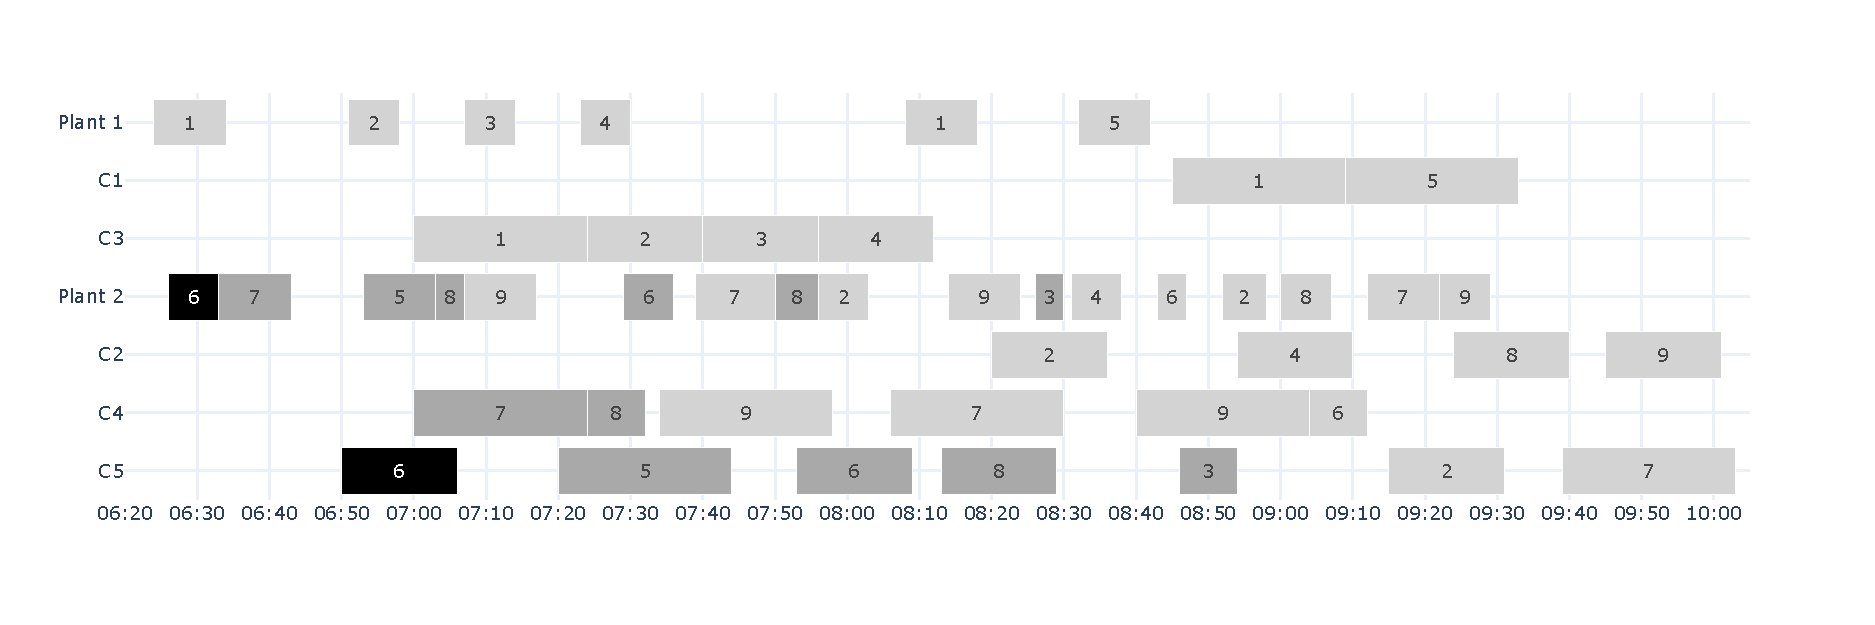
\includegraphics[width=\linewidth]{exemple.pdf}
\end{figure}

\section{Constructive heuristics and GRASP}
\label{sec:cdp_grasp_method}

This section presents the heuristic approach to solving the Concrete Delivery Problem. Our method consists of constructing feasible solutions of the CDP with randomized greedy heuristics and iteratively invoking these heuristics in the GRASP metaheuristic. From now on, we represent the scheduling of a delivery node $d$ as the pair ($L^k_{d}$,$U^k_{d}$) of loading and unloading tasks. $L^k_{d} = \left(b,q_d,v_b,w_b\right)$ indicates that driver $k$ will load $q_d$ $m^3$ of RMC at plant $b$ between timeslots $\left[v_b,w_b\right]$ to serve $d$. $U^k_{d} = \left(k,v_d, w_d\right)$ indicates that driver $k$ will start unloading at time $v_d$ and finish at time $w_d$. We then call a solution $Sol =\left\lbrace \cup _{1 \leq j \leq |D|} (L^k_{j}, U^k_{j}), k \in K \right\rbrace$ the set of all pairs of loading and unloading tasks performed on a given day.

\subsection{GRASP algorithm}

The Greedy Randomized Search Procedure (GRASP) algorithm is a multi-start metaheuristic for combinatorial optimization problems proposed by \cite{feo1989probabilistic}. It is a two-phase iterative sequence of constructive and local search algorithms. A feasible solution is generated in the construction phase using a greedy randomized algorithm. Then, a local search phase tries to improve it. Algorithm~\ref{alg_grasp} outlines the GRASP algorithm. We start with a list of greedy randomized heuristics and iterate on each to construct an incumbent solution $Sol$ on which we apply a local search procedure to explore its neighborhood. The best solution found so far is then stored. To avoid redundant computations, a hash table $T$ ensures that the local search is not applied twice to the same solution. The procedure stops and returns the best overall solution when certain stopping conditions are met, such as reaching a time limit or a maximum number of iterations. 
    \begin{algorithm}[hbpt]
        \caption{Pseudo-code of the GRASP algorithm }
        \label{alg_grasp}
        \DontPrintSemicolon
        \LinesNumbered
        \setcounter{AlgoLine}{0}
        \KwIn{ \textit{H}: List of constructive greedy randomized heuristics }
        $Sol^{*} \leftarrow \emptyset$    \hspace{2mm}        $Cost(Sol^*) \leftarrow \infty$

        Initialize an empty hash table $T \leftarrow \emptyset$

        % $counter \leftarrow  0$

        \While{conditions not met}{

            \ForEach{$heuristic \in H$}{
                $Sol \leftarrow heuristic()$

                \uIf{ $Sol \notin T$}{
                    $Sol \leftarrow LocalSearch(Sol)$

                    Add $Sol$ to $T$

                    \uIf{$Cost(Sol)< Cost(Sol^*)$}{
                    $Sol^* \leftarrow Sol$
                    }
                }
            }
        }

        \KwRet{$S^{*}$}
    \end{algorithm}
            
For the construction phase, we developed two greedy randomized heuristics: the customer-based insertion with backtracking, which schedules customers one at a time, and the delivery-based insertion.%, which does not necessarily complete the scheduling of one customer before starting to schedule another.
% The greedy aspect of GRASP is the creation of the set $RCL$, the probabilistic aspect is the random selection in $RCL$, and the adaptive aspect is the updating of $CL$ and the re-evaluation of the incremental costs.

\subsection{Customer-based insertion with backtracking heuristic}

The customer-based insertion heuristic builds a solution from scratch by iteratively scheduling one customer at a time. When a customer is selected, all deliveries needed to serve that customer are scheduled before moving on to the next customer. As shown in Algorithm~\ref{alg:greedyCustIns}, between lines $4$ and $38$, we iterate over a shuffled list of orders for each customer.

To schedule an order $o$, we begin with its first delivery node. Once this node is scheduled, we proceed to schedule the subsequent delivery nodes until $o$ is completely served. For each delivery node $d$, the algorithm identifies between lines $9$ and $12$ each driver capable of visiting this node using the $SimulateVisit$ procedure. For all drivers able to serve $d$, at line $12$ we store the details about the pair of loading and unloading tasks and its cost in $M[d]$.

If at least one driver can serve the node (line $13$), we randomly select at line $16$  a pair of loading and unloading tasks whose cost falls within a specified range based on a parameter $\theta$ and insert this pair into $Sol$ at line $18$. Then we update the order remaining demand and proceed with the next delivery node at line $19$. 

In cases where no driver can visit the node $d$, the algorithm employs a backtracking scheme to address two distinct scenarios. First, if the visit to $d$ cannot be scheduled due to cold-joint constraints (i.e., the time between consecutive deliveries exceeds $\gamma^1$), the $DelayPreviousDelivery$ procedure is employed. This procedure determines if a previous delivery $D^{j'}_o$ of the same order exists such that $d$ can be successfully scheduled in the current solution by delaying the start of service of $D^{j'}_o$ by $\lambda$. If $D^{j'}_o$ exists, the schedules of all delivery nodes between $D^{j'}_o$ and $d$ are removed, and the scheduling of order $o$ resumes from $D^{j'}_o$. 

The procedure $DelayPreviousDelivery$ computes the difference $\lambda$ between the earliest time a driver can visit $D^{j}_o$ and the end of service of its immediate predecessor node $D^{j-1}_o$. Then, it tries to find one of the precedent nodes of $D^{j}_o$ for which we can delay the start of service of at least $\lambda = min(\lambda,\gamma^1)$. If such a node exists, the procedure returns it and the value of the delay. Then we backtrack to this node and restart the scheduling process.

In cases where infeasibility arises from other violated constraints, the algorithm attempts to backtrack to a precedent node and retry the scheduling with another driver. At line $31$, the algorithm searches for the first precedent node $D^{j'}_o$ with remaining pair of tasks in $M[D^{j'}_o]$. If found, the schedules of all delivery nodes between $D^{j'}_o$ and $d$ are removed, and backtracking occurs to $D^{j'}_o$. In this iteration, since $M[D^{j'}_o]$ is not empty, the $SimulateVisit$ procedure is not called again; instead the stored elements of $M[D^{j'}_o]$ are utilized.

If no precedent node suitable for backtracking is found, it indicates that the current customer cannot be scheduled. Consequently, all previously scheduled visits to its delivery nodes are removed before advancing to the next customer (as described in lines $23$--$25$ and lines $32$--$34$). The procedure stops when all customers are evaluated and returns the constructed solution $Sol$ at the end.

The $SimulateVisit$ procedure takes a partial solution, a delivery node $d$, a driver $k$ and the delay value $\lambda$ as parameters. Its goal is to find the earliest time when the loading service for $d$ can start at its home plant $b$. When planning to visit delivery node $d$ of order $o$ and customer $c$ with driver $k$, we first compute his delivery time $v_d$ as follows. If $d$ is the first  visited node of customer $c$, then we expect its service to start at $v_d = a_c + \lambda$. Otherwise, if the previous node $j$ visited before $d$ belongs to the same order $o$, then the service at $d$ may begin at the random value $w_j + rand(\lambda, \gamma^1)$ to respect the allowed time between two consecutive deliveries of the same order. We randomize $v_d$ to allow more diversity in our solution space. Finally, if $j$ and $d$ belong to different orders, then $v_d = w_j + rand(0,\gamma^2)$.

Let $\bar{q}_o$ be the remaining demand of order $o$. Driver $k$ can supply $d$ with the quantity $q^k_d= \min(\bar{q}_o,Q^k)$. We determine the loading start time $v_l$ of the corresponding dock node $l$ by subtracting the travel time, adjustment time, and loading duration from $v_d$: $w_l = v_d - t_{dl} - \alpha_b - q^k_{d}/\tau^l{_b} $. If $j$ is the last node where $k$ was unloading with a service duration $s_j$, then $w_l= \max(w_l, v_j + s_{j} + t_{jl})$. Now, we have the earliest time $k$ can start loading at plant $b$, but if the loading dock is occupied at that time, $k$ will have to wait. To find the real loading time, we use a data structure that stores all timeslots when a plant is occupied. Then, starting from $w_l$, we search forward for the first timeslot with duration $q^k_{d}/\tau^l{_b}$ where we can insert this loading operation and update $w_l$ accordingly. Changing $w_l$ can cause violations of the time window or cold-joint constraints, especially for an order's subsequent deliveries, and thus make the schedule infeasible. So with this new value of $w_l$, we recompute $v_l$ and check for constraint violations.

Algorithm~\ref{alg:greedyCustIns} is designed with a list of customers as input. Initial experimentation has revealed that the sequence of this list affects the final solution. Within the GRASP framework, we invoke the customer-based heuristic multiple times with various customer orderings. These include sorting by decreasing demand and time window, sorting by increasing demand and time window, and finally, with a randomized list.
    \begin{algorithm}[!ht]
        \caption{Customer-based insertion algorithm }
        \label{alg:greedyCustIns}
        \DontPrintSemicolon
        \LinesNumbered
        \setcounter{AlgoLine}{0}
        \KwIn{  $Sol$: empty solution, $K$: vehicles set, $\Pi$: list of customers }

        $M \leftarrow \emptyset $ \tcp{List of pairs of loading -- unloading tasks for each delivery node}

        \ForEach{$c \in \Pi$}{

            Shuffle $ O_c$

            \ForEach{$o \in O_c$}{

                $\lambda \leftarrow 0$, $\bar{q}_o\leftarrow q_o$, $j \leftarrow 1$

            \While{$\bar{q}_o>0$}{

                $d \leftarrow D^j_{o}$

                \uIf{($M[d] = \emptyset $) or ($\lambda >0$)}{

                    \ForEach{ $k \in K$  }{

                        $(L^k_{d}$, $U^k_{d},cost,f)$ $\leftarrow $ SimulateVisit($Sol$,$d$,$k$,$\lambda$)

                        \uIf{f=1}{
                                $M[d] \leftarrow M[d] \cup \{(L^k_{d}, U^k_{d},cost,k)\}$ 
                            }
                    }
                }

                \uIf{$M[d]\neq \emptyset$}{

    $c_{min} \leftarrow \min\left\{ cost \ | \ (L^k_{d}, U^k_{d},cost,k) \in M[d]   \right\} $

    $c_{max} \leftarrow \max\left\{ cost \ | \ (L^k_{d}, U^k_{d},cost,k) \in M[d]   \right\} $
    
    Randomly choose $(L^k_{d}, U^k_{d},cost,k)$ in $M[d]$ such that $cost \leq c_{min} + \theta (c_{max}-c_{min}) $

    $M[d]\leftarrow M[d] \backslash \{(L^k_{d}, U^k_{d},cost,k)\} $
    
    $Sol \leftarrow Sol \cup \{(L^k_{d}$, $U^k_{d})\}  $

        $\bar{q}_o \leftarrow \bar{q}_o-q^k_{d}$, $\lambda \leftarrow 0$, $j \leftarrow j+1$

    }
    \uElse{
        \uIf{cold-joint constraints}{
            $(D^{j'}_o,delay)$ = $DelayPreviousDelivery$($Sol$,$d$) \tcp{$j'<j$}

        \uIf{no $D^{j'}_o$ exists}{

            $Sol \leftarrow Sol \backslash \{(L^k_{i}, U^k_{i}), \forall i \in D_c\}$

            Go to line 2 \tcp{continue with next customer}
}

$Sol \leftarrow Sol \backslash \{(L^k_{i}, U^k_{i}), \forall i \in (D^{j'}_{o},..,D^{j-1}_{o})  \}$

Update $\bar{q}_o$

$j \leftarrow j'$, $\lambda \leftarrow delay$

    Go to line 6 \tcp{backtrack to $j'$ position and retry to insert $D^{j'}_{o}$}
    }
    \uElse{
     Search for a precedent delivery node $D^{j'}_o, j'<j$ with $M[D^{j'}_o]\neq \emptyset$

    \uIf{ no $D^{j'}_o$ exists}{

    $Sol \leftarrow Sol \backslash \{(L^k_{i}, U^k_{i}), \forall i \in D_c\}$

    Go to line 2 \tcp{continue with next customer}
    }

    $Sol \leftarrow Sol \backslash \{(L^k_{i}, U^k_{i}), \forall i \in (D^{j'}_{o},..,D^{j-1}_{o})  \}$

    Update $\bar{q}_o$

     $j \leftarrow j'$

    Go to line 6 \tcp{backtrack to precedent delivery node $D^{j'}_o$ }
                        }

                    }
                    
                }
            }
        }
        \KwRet{$Sol$}
    \end{algorithm}

When confronted with scenarios where several customers require their services to start simultaneously or within the same time window, we observed that with Algorithm~\ref{alg:greedyCustIns}, some customers remain unscheduled when resources are limited. To address this limitation, we introduce the delivery-based insertion heuristic.

\subsection{Delivery-based insertion heuristic}

The delivery-based insertion heuristic (Algorithm~\ref{alg:delbasedIns}) iteratively constructs a solution from scratch by scheduling one delivery node at a time. The algorithm starts with an empty solution $Sol$ and initially fills a candidate list $CL$ with the first node of a randomly selected order for each customer. Within each iteration of the $while$ loop, the algorithm filters $CL$ to obtain a reduced candidate list $CL'$ of deliveries based on a specified criterion, such as prioritizing deliveries with the highest (lowest) demands, earliest (latest) due dates, or lowest order numbers. This filtering is performed by the $Filter$ procedure, allowing the algorithm to explore different neighborhoods. Thus, within the GRASP framework, we can invoke the delivery-based heuristic multiple times with different filtering procedures which evaluate different neighborhoods. 

Between lines $14$ and $18$, for each delivery $d$ in $CL'$, the algorithm determines the best available driver $k$ who can visit it. Then, the corresponding pair of loading and unloading tasks $(L^k_d, U^k_d)$, along with its costs, are stored in $M[d]$. This is done using the $SimulateVisit$ procedure described earlier. Then, the algorithm constructs at line $20$ a list $T$ containing all pairs of loading and unloading tasks for the delivery nodes in $CL'$.

If $T$ is empty, the algorithm assumes that the customers associated with the nodes in $CL'$ cannot be scheduled, and it removes those customers' existing schedules from the solution. It then excludes $CL'$ from $CL$ at line $25$ and proceeds to the next iteration.

Otherwise, from line $26$ to line $29$, the algorithm randomly selects from $T$ a pair of loading and unloading tasks whose cost falls within a specified range determined by the parameter $\theta$ and inserts this pair into $Sol$. The algorithm then updates the remaining orders and customer quantities and excludes the scheduled delivery node from $CL$. If an order $o$ is not completely fulfilled after visiting $d^j_{o}$, the next delivery node $d^{j+1}_{o}$ is added to $CL$.  Otherwise, if the customer has remaining orders, the first delivery node $d^{1}_{o'}$ of another randomly selected order $o'$ is added to $CL$.

Unlike the customer-based insertion, the delivery-based insertion allows each customer to have one of its delivery nodes considered for scheduling at each iteration.
%In these two heuristics, the greedy aspect of GRASP refers to the creation of the set $RCL$, the probabilistic aspect is the random selection in $RCL$, and the adaptive part is the updating of $CL$ and the re-evaluation of the costs.
 
\begin{algorithm}[!ht]
    \caption{Delivery-based insertion algorithm }
    \label{alg:delbasedIns}
    \DontPrintSemicolon
    \LinesNumbered
    \setcounter{AlgoLine}{0}
    \KwIn{  $Sol$: empty solution, $\Pi$: list of customers, $Filter$: filtering procedure}

    $CL \leftarrow \emptyset$

    $M \leftarrow \emptyset $ \tcp{List of pairs of loading -- unloading tasks for each delivery node}

    $\bar{q} \leftarrow \emptyset$ \tcp{List of remaining demands}

    \ForEach{$c \in \Pi$}{
        $\bar{q}_c \leftarrow q_c$

        Select a random order $o \in O_c$

        $CL \leftarrow CL \cup \{d^1_{o}\}$

        $\bar{q}_o \leftarrow q_o$
    }

    \While{$CL \neq \emptyset$}{

        $CL' \leftarrow \text{} Filter (CL) $

        $T \leftarrow \emptyset $ \tcp{List of loading and unloading tasks}

        \ForEach{ $d \in CL'$}{

            $best\_cost \leftarrow +\infty$

            \ForEach{ $k \in K$  }{

                $(L^k_{d}$, $U^k_{d},cost,f)$ $\leftarrow $ SimulateVisit($Sol$,$d$,$k$,$\lambda$)

                \uIf{f=1 and $cost <       best\_cost$}{
                    $M[d] \leftarrow \{(L^k_{d}, U^k_{d},cost,k)\}$ 

                    $best\_cost \leftarrow c$
                }
            }

            \uIf{$M[d]\neq \emptyset$}{
                $T \leftarrow T \cup M[d]$    
            }
        }
        \uIf{$T = \emptyset$}{
            \ForEach{$d \in CL'$}{
            
           $c \leftarrow $ customer associated with $d$

            $Sol \leftarrow Sol \backslash \{(L^k_j,U^k_j), \forall j \in D_c \}$
           }
           $CL \leftarrow CL\backslash CL'$ 
        }
        \uElse{
            $c_{min} \leftarrow \min\left\{ cost \ | \ (L^k_{d}, U^k_{d},cost,k) \in T   \right\} $

            $c_{max} \leftarrow \max\left\{ cost \ | \ (L^k_{d}, U^k_{d},cost,k) \in T   \right\} $
    
            Randomly choose $(L^k_{d^j_o}, U^k_{d^j_o},cost,k) \in T$ such that $cost \leq c_{min} + \theta (c_{max}-c_{min}) $
            
            $Sol \leftarrow Sol \cup \{(L^k_{d^j_o}$, $U^k_{d^j_o})\} $

            $\bar{q}_o \leftarrow \bar{q}_o-q^k_{d^j_o}$, $\bar{q}_c \leftarrow \bar{q}_c-q^k_{d^j_o}$ \tcp{$o \in O_c$}

            $CL \leftarrow CL \backslash \{d^{j}_o\}$

            \uIf {$\bar{q}_{o} \neq 0$ }{

                $CL \leftarrow CL \cup \{d^{j+1}_{o}\}$
            }
            \uElseIf{ $\bar{q}_c \neq 0$}{

                Select another order $o' \in O_c$

                $CL \leftarrow CL \cup \{d^{1}_{o'}\} $
            }

        }      
    }
        \KwRet{$Sol$}
\end{algorithm}

\subsection{Local Search}

After the construction phase, the local search phase invokes local search operators to either repair or improve the incumbent. One operator is used to repair a solution where not all customers are scheduled. Then four operators are used to improve the incumbent using a first-improvement strategy. The local search continues until no more improvements can be made or a timeout is reached. 

\subsubsection{Repair operator}

The Remove and Reschedule operator is used to address situations where a solution contains unscheduled customers. This operator first selects an unscheduled customer $c$ from the solution and identifies a set $\Pi_c$ containing scheduled customers sharing the same time slot with $c$. The schedules of all elements of $\Pi_c$ are then removed from the solution and retried to be scheduled again along with $c$. 

\subsubsection{Improvement operators}

The first improvement or Load Backward operator is used when dealing with solutions containing customers whose first delivery is late. In such cases, the goal is to schedule the loading start time for the first delivery node for these customers as early as possible. This operator is implemented by iterating backward through the timeslots data structure when calculating the loading start time within the $SimulateVisit$ procedure. By doing so, the operator aims to find a loading start time that allows for earlier delivery, thus reducing the late first delivery cost. The other improvement operators are based on the swap and relocate moves. 

We have implemented two moves based on the swap operator. The Swap Driver operator explores alternative driver assignments by swapping drivers assigned to two delivery nodes. This allows for the assessment of different driver configurations, potentially leading to improvements in solution quality. The Swap Load operator exchanges loads between a delivery node and the last delivery node of the same order. In our greedy randomized heuristics, all deliveries of an order are typically filled to capacity, except for the last one.  This operator investigates the effect of delivering this last load much earlier in the delivery sequence. Delivering the final load earlier in the sequence can improve the loading operations, as it may be easier to find an empty timeslot for inserting a loading task with a smaller load. 

We also implemented two moves based on the relocate operator. The Consolidate Load operator is applied on an order with a remaining demand between $]Q_{min},Q_{max}]$. If this remaining demand is served with two drivers with capacity $Q_{min}$, then the operator tries to consolidate it to be served by a single driver with a capacity of $Q_{max}$. Next, the Relocate Driver operator removes a delivery node from its current route and inserts it in another driver's route. This enables the redistribution of delivery nodes among drivers, potentially reducing drivers underutilization and overtime costs.

\section{Computational experiments}
\label{sec:cdp_comp_exp}

In this section, we present and discuss the results of computational experiments conducted using the GRASP heuristic described in Section~\ref{sec:cdp_grasp_method}. The implementation of the GRASP algorithm is coded in C++. We run our experiments on the benchmark data used in \cite{kinable2014concrete}, and on a new dataset extracted from delivery operations records provided by our industry partner.

\subsection{Generation of instances}
\newcommand{\nbInstance}{35}
The dataset used in this section was obtained from our partner and contains records representing delivery operations from up to 8 plants for $\nbInstance$ days. From this historical data, we extracted information such as daily orders delivered, plant assignments to orders, and the number of available drivers. We created $\nbInstance$ instances from this data, where each instance corresponds to a daily operation. To maintain confidentiality, we have removed the GPS coordinates of customers and plants but have included two matrices containing the distances and driving times between all plants and customers. An instance contains information such as each driver's capacity, associated batch plant, and shift start time (which we generate). For each customer, we have the due time, the total demand, the number of orders (type of concrete) received, and its index in the time (distance) matrix. For each order, we have its demand and the corresponding customer and production plant. Finally, we have the loading capacity for each plant, as well as its index in the time matrix. The name of an instance has the format $C\_n\_o\_k\_p$, where $n$ is the number of customers, $o$ is the total number of orders, $k$ is the number of available drivers, and $p$ is the number of plants. The dataset is divided into small, medium, and large sets according to the total number of daily orders. We have summarized the dataset in Table~\ref{tab:cdp_instances}. The small dataset has eight instances with four to eleven customers whose demands vary between 226.5 and 937.5 m$^3$. These customers request between 7 and 14 orders, which are served from one to three depots with a fleet of 13 to 35 concrete mixers. The dataset is available online at \url{https://sites.google.com/view/jfcote/} as a contribution to the CDP literature.
\begin{table}[htpb]
    \centering
    \caption{Instances summary}
    \label{tab:cdp_instances}
    \resizebox*{0.9\textwidth}{!}{
        \begin{tabular}{lcccccc}
            \toprule
            {}     & \# & Demand (m$^3$)           & \#Orders   & \#Customers & \#Drivers & \#Depots \\
            \midrule
            Small  & 8  & 226.5 -- 937.5     & 7 -- 14    & 4 -- 11   & 13 -- 35    & 1 -- 3     \\
            Medium & 14 & 1,160.5 -- 2,971.0 & 43 -- 98   & 40 -- 89  & 76 -- 137   & 6 -- 8     \\
            Large  & 13 & 3,078.5 -- 3,953.5  & 107 -- 136 & 92 -- 114 & 129 -- 149  & 8       \\
            \bottomrule
        \end{tabular}
    }
\end{table}

\subsection{Results for the instances of \cite{kinable2014concrete}}

\cite{kinable2014concrete} provided a benchmark dataset for their variant of the CDP. Although their primary objective is to maximize the total load delivered each day without considering loading operations at a plant and ensuring deliveries within specified time windows, we still use this dataset to analyze and compare the performance of our algorithm under different conditions. \cite{kinable2014concrete} solved their problem with a CP algorithm, MIP, steepest descent heuristic (SD), and fix-and-optimize MIP heuristic (MIP fix \& opt), which is a hybridization of the MIP and SD. They also provide dual bounds to help assess the optimality of the instances. Table \ref{tab:cdp_lit_comp} shows the performance of the GRASP heuristic against the methods mentioned above. For each method, the table shows the average execution time in seconds and the corresponding gap between the obtained solution and the dual bound provided by \cite{kinable2014concrete}. The row Opt reports the number of optimal solutions found by each method.

\begin{table}[htbp]
    \centering
    \caption{Performance of the GRASP heuristic on the CDP benchmark instances}
    \label{tab:cdp_lit_comp}
    \scriptsize
    \resizebox{1\textwidth}{!}{
        \begin{tabular}{@{}cccccccccc|cc@{}}
            \toprule
            & &  \multicolumn{8}{c}{\cite{kinable2014concrete}} & \multicolumn{2}{|c}{Our paper} \\
            \cmidrule(l){3-10} \cmidrule(r){11-12}
             &     & \multicolumn{2}{c}{CP}     & \multicolumn{2}{c}{MIP}   & \multicolumn{2}{c}{SD-heuristic} & \multicolumn{2}{c}{MIP fix \& opt} & \multicolumn{2}{|c}{GRASP}                                                 \\ \cmidrule(l){3-10} \cmidrule(r){11-12}
               &     & Gap (\%)                   & Time (s)                 & Gap (\%)                         & Time (s)                  & Gap (\%)                   & Time (s) & Gap (\%) & Time (s) & Gap (\%) & Time (s) \\ \cmidrule(l){3-10} \cmidrule(l){11-12}
            \multirow{2}{*}{Set A} & Avg & 4.2                        & 196.95                  & 7.3                              & 149.14                 & 9.1                        & 0.02        & 7.0      & 100.70   & 5.7      & 13.18    \\ \cmidrule(l){2-10} \cmidrule(r){11-12}
                & Opt & \multicolumn{2}{c}{40/64}  & \multicolumn{2}{c}{37/64} & \multicolumn{2}{c}{30/64}        & \multicolumn{2}{c|}{35/64}  & \multicolumn{2}{c}{35/64}                                                            \\ \cmidrule(l){3-10} \cmidrule(r){11-12}
            \multirow{2}{*}{Set B} & Avg & 12.1                       & 355.95                   & -                                & -                          & 16.3                       & 1.33     & -        &  \multicolumn{1}{c|}{-}         & 13.8     & 574.98   \\ \cmidrule(l){2-10} \cmidrule(r){11-12}
              & Opt & \multicolumn{2}{c}{55/128} & \multicolumn{2}{c}{-}     & \multicolumn{2}{c}{40/128}       & \multicolumn{2}{c|}{-}      & \multicolumn{2}{c}{44/128}                                                           \\ \bottomrule
        \end{tabular}
    }
\end{table}

Overall, our GRASP algorithm shows its effectiveness in providing good and competitive solutions in a relatively short time for this benchmark of the CDP, making it a suitable candidate for further analysis and real-world application.  It outperformed all methods except CP, achieving an average gap of 5.7\% (13.8\%) with a runtime of 13 (575) seconds for Set A (Set B). The SD-heuristic appears to be much faster (23 milliseconds for set A), but GRASP provides a better balance between solution quality and computation time. It should also be noted that the exact MIP, CP, and MIP fix \& opt are initialized with the results of the SD-heuristic.

\subsection{Results for the generated instances}

The computational results of our instances solved with the GRASP heuristic are summarized in the tables below. The parameters used in our experiments are listed in Table~\ref{tab:cdp_problem_parameters}.

\begin{table}[!ht]
    \centering
    \caption{Parameters of the real-world instances}
    \label{tab:cdp_problem_parameters}
    \small
    \begin{tabularx}{\textwidth}{Xr}
        \toprule
        \multicolumn{1}{c}{Parameter}  &
        \multicolumn{1}{c}{Value} \\ \midrule
 Time window ($\tau^w$)  & 60 min    \\
 Unloading duration ($\tau_c^u$)  & 2 min$/m^3$   \\
 Cleaning duration ($\rho$)    & 10 min  \\
        Adjustment duration ($\alpha$)                                                & 10 min                    \\
        Max travel time ($\Delta$)                                                    & 120 min                   \\
        Min working time ($\mu$)                                                      & 180 min                   \\
        Max working time ($\eta$)                                                      & 480 min                   \\
        Max overtime duration ($\varLambda$)                                                 & 120 min                   \\
        Max delay between two consecutive deliveries of the same order $\gamma^1$)   & 20 min                    \\
        Max delay between two consecutive deliveries of different orders ($\gamma^2)$ & 25 min                    \\
        Penalty of unfulfilled orders ($\beta_1$)                                     & 100,000                   \\
        Penalty of first delivery delay ($\beta_2$)                                   & 10,000                    \\
        Penalty for driver underutilization  ($\beta_3$)                              & 30                        \\
        Driver overtime penalty $ (\beta_4$)                                          & 20                        \\
        \bottomrule
    \end{tabularx}
\end{table}

Table \ref{tab:cdp_all_instances} contains the detailed results for all instances with a stop criterion of 3600 seconds. The table shows the demand of each instance, the average, and the best values of the objective function when solving each instance five times. All daily orders of the small instances are completely served by our algorithm within these five iterations, as shown in column $UQ$, which reports the undelivered quantities. For the medium and large instances, $99.5\%$ and $99.6\%$ of the total demands are delivered. The sum of driver underutilization costs ($DUC$) is high for medium and large instances. This indicates the underutilization of the scheduled fleet. Some drivers are not scheduled at all or work very little. The sum of driver overtime costs ($DOC$) is also high for these instances. This can be explained by the fact that the algorithm prioritizes drivers on overtime rather than using a driver who has to travel to another plant for a delivery, which would increase travel costs ($TC$).

$FDD$ represents the sum of the delays of the first deliveries. In the case of small instances, all but one of the first deliveries are on time. However, for the other instance sets, there is at least one customer with a late first delivery. To provide insight into the actual delay experienced by customers, we report $mFDD$, which is the maximum delay among all first deliveries. This information reveals that for small instances, the maximum delay ranges between 0 and 35.7 minutes. For medium instances, it varies from 32.7 to 60 minutes, and for large instances, it falls within the range of 56 to 60 minutes.

\begin{table}[ht!]
    \centering
    \caption{Results with all instances}
    \label{tab:cdp_all_instances}
    \resizebox{\textwidth}{!}{
    \begin{tabular}{lcccccrrrrrrrrrrrrr}
    \toprule
     &  &  &  & & & \multicolumn{6}{c}{Avg} & \multicolumn{7}{c}{Best}  \\
    \cmidrule(l){7-12} \cmidrule(l){13-19}
     &  &  &  &  & \multicolumn{1}{c}{Demand}  & \multicolumn{1}{c}{$TC$}& \multicolumn{1}{c}{$UQ$} & \multicolumn{1}{c}{$FDD$} & \multicolumn{1}{c}{$DUC$} & \multicolumn{1}{c}{$DOC$} & \multicolumn{1}{c}{\multirow[c]{2}{*}{Z}}  & \multicolumn{1}{c}{($TC$)} & \multicolumn{1}{c}{$UQ$} & \multicolumn{1}{c}{$FDD$} & \multicolumn{1}{c}{$mFDD$} & \multicolumn{1}{c}{$DUC$} & \multicolumn{1}{c}{$DOC$} & \multicolumn{1}{c}{\multirow[c]{2}{*}{Z}}  \\
      & |$C$| & $|O|$ & $|K|$ & $|B|$ & \multicolumn{1}{c}{(m$^3$)}& \multicolumn{1}{c}{(min)} & \multicolumn{1}{c}{(m$^3$)} & \multicolumn{1}{c}{(min)} & \multicolumn{1}{c}{(min)} & \multicolumn{1}{c}{(min)} &  & \multicolumn{1}{c}{(min)} & \multicolumn{1}{c}{(m$^3$)} & \multicolumn{1}{c}{(min)} & \multicolumn{1}{c}{(min)} & \multicolumn{1}{c}{(min)} & \multicolumn{1}{c}{(min)} &  \\
    \midrule
    \multirow[c]{8}{*}{Small} & 11 & 12 & 13 & 1 & 226.5 & 1,243.5 & 0.0 & 0.0 & 18.8 & 0.0 & 1,807.7 & 1,243.5 & 0.0 & 0.0 & 0.0 & 0.0 & 0.0 & 1,243.5 \\
    & 5 & 8 & 13 & 1 & 267.0 & 745.1 & 0.0 & 0.0 & 0.0 & 0.0 & 745.1 & 745.1 & 0.0 & 0.0 & 0.0 & 0.0 & 0.0 & 745.1 \\
    & 6 & 11 & 18 & 2 & 333.5 & 753.3 & 0.0 & 0.0 & 255.9 & 0.0 & 8,430.6 & 753.3 & 0.0 & 0.0 & 0.0 & 176.0 & 0.0 & 6,034.2 \\
    & 4 & 7 & 15 & 2 & 375.0 & 1,017.5 & 0.0 & 0.0 & 218.2 & 131.3 & 10,190.9 & 1,017.6 & 0.0 & 0.0 & 0.0 & 82.8 & 33.9 & 4,179.8 \\
    & 7 & 8 & 19 & 2 & 388.0 & 1,790.5 & 0.0 & 0.0 & 318.4 & 137.8 & 14,119.2 & 1,817.0 & 0.0 & 0.0 & 0.0 & 52.6 & 98.7 & 5,368.6 \\
    & 10 & 14 & 29 & 3 & 613.5 & 3,482.1 & 0.0 & 59.5 & 239.4 & 373.5 & 77,635.1 & 3,513.2 & 0.0 & 59.5 & 35.7 & 147.2 & 304.0 & 73,510.2 \\
    & 8 & 11 & 31 & 3 & 776.0 & 2,325.7 & 0.0 & 0.0 & 796.3 & 690.1 & 40,015.9 & 2,311.7 & 0.0 & 0.0 & 0.0 & 593.7 & 601.0 & 32,141.2 \\
    & 9 & 10 & 35 & 3 & 937.5 & 4,110.9 & 0.0 & 0.0 & 447.7 & 712.0 & 31,782.1 & 4,139.9 & 0.0 & 0.0 & 0.0 & 243.3 & 550.0 & 22,439.9 \\
     \cmidrule(l){1-12} \cmidrule(l){13-19}
     \multicolumn{5}{r}{Average} & \multicolumn{1}{c}{-} & 1,933.6 & 0.0 & 7.4 & 286.8 & 255.6 & 23,090.8& 1942.7&0.0&7.4&4.5&161.9&198.5&18,207.8\\
     \cmidrule(l){1-12} \cmidrule(l){13-19}
     \multirow[c]{14}{*}{Medium} & 40 & 43 & 76 & 6 & 1,160.5 & 6,085.6 & 0.0 & 44.8 & 3,017.6 & 1,140.3 & 164,186.8 & 6,451.5 & 0.0 & 32.7 & 8.5 & 2,714.0 & 899.1 & 138,530.5 \\
 & 42 & 47 & 104 & 8 & 1,565.0 & 8,024.3 & 12.0 & 55.5 & 3,563.0 & 160.2 & 1,373,593.7 & 8,106.6 & 12.0 & 54.7 & 16.8 & 3,358.8 & 138.7 & 1,366,363.9 \\
 & 63 & 70 & 94 & 7 & 1,746.5 & 13,871.4 & 0.0 & 228.2 & 1,250.1 & 1,398.4 & 307,504.3 & 13,902.5 & 0.0 & 195.3 & 58.9 & 1,465.1 & 1,206.7 & 277,317.6 \\
 & 67 & 78 & 116 & 8 & 1,839.5 & 13,225.9 & 0.0 & 142.1 & 1,931.4 & 751.0 & 228,250.5 & 13,460.9 & 0.0 & 139.3 & 33.8 & 935.5 & 962.9 & 200,057.2 \\
 & 71 & 82 & 116 & 8 & 2,060.0 & 11,158.1 & 9.0 & 263.3 & 2,797.8 & 982.1 & 1,277,996.2 & 10,748.5 & 9.0 & 243.3 & 45.9 & 2,218.9 & 594.8 & 1,232,488.4 \\
 & 57 & 70 & 117 & 6 & 2,327.5 & 14,551.7 & 0.0 & 322.2 & 1,654.3 & 1,566.4 & 417,729.4 & 14,732.0 & 0.0 & 252.5 & 49.5 & 1,438.4 & 1,551.1 & 341,397.0 \\
 & 79 & 83 & 137 & 7 & 2,425.0 & 17,886.5 & 0.0 & 663.2 & 2,132.2 & 2,031.5 & 785,718.4 & 17,555.1 & 0.0 & 559.6 & 58.6 & 1,707.6 & 2,159.2 & 671,538.1 \\
 & 66 & 80 & 127 & 8 & 2,512.5 & 15,108.4 & 0.0 & 118.4 & 1,600.3 & 1,596.7 & 213,496.4 & 14,567.4 & 0.0 & 114.1 & 34.3 & 1,349.9 & 1,143.2 & 191,985.5 \\
 & 68 & 74 & 128 & 7 & 2,595.0 & 18,744.1 & 1.6 & 547.5 & 1,238.4 & 2,827.7 & 822,423.5 & 18,276.6 & 0.0 & 355.6 & 55.8 & 1,206.4 & 3,061.4 & 471,318.0 \\
 & 85 & 97 & 136 & 8 & 2,673.0 & 17,252.5 & 0.0 & 427.7 & 2,085.1 & 2,355.1 & 554,640.8 & 18,164.5 & 0.0 & 361.0 & 53.3 & 1,447.8 & 2,081.4 & 464,253.2 \\
 & 78 & 85 & 128 & 8 & 2,685.5 & 15,931.9 & 63.0 & 461.4 & 1,243.9 & 2,783.1 & 6,870,259.9 & 16,164.5 & 63.0 & 391.1 & 57.8 & 1,553.3 & 2,371.0 & 6,801,308.3 \\
 & 77 & 85 & 131 & 8 & 2,893.5 & 17,168.9 & 0.0 & 410.7 & 1,360.1 & 1,756.7 & 503,850.9 & 17,620.2 & 0.0 & 388.1 & 57.5 & 963.2 & 2,149.1 & 477,607.4 \\
 & 89 & 97 & 137 & 7 & 2,939.5 & 21,350.0 & 13.4 & 865.0 & 1,074.2 & 3,247.2 & 2,327,223.6 & 21,551.0 & 0.0 & 880.5 & 47.7 & 1,318.9 & 3,375.7 & 1,009,098.9 \\
 & 84 & 98 & 133 & 7 & 2,971.0 & 20,620.2 & 39.2 & 1,091.8 & 736.8 & 2,666.4 & 5,106,602.3 & 20,578.3 & 31.5 & 887.0 & 59.1 & 839.1 & 2,910.7 & 4,141,019.3 \\
     \cmidrule(l){1-12} \cmidrule(l){13-19}
     \multicolumn{5}{r}{Average} & \multicolumn{1}{c}{-} & 15,070.0 & 9.9 & 403.0 & 1,834.7 & 1,804.5 & 1,496,676.9& 15,134.3&8.2&346.8&45.5&1,608.4&1,757.5&1,270,305.9\\
    \cmidrule(l){1-12} \cmidrule(l){13-19}
    \multirow[c]{14}{*}{Large} & 98 & 109 & 132 & 8 & 3,078.5 & 22,498.9 & 0.0 & 456.2 & 457.4 & 3,961.9 & 571,626.0 & 22,359.3 & 0.0 & 394.4 & 56.2 & 463.1 & 3,905.6 & 508,725.2 \\
 & 101 & 119 & 129 & 8 & 3,229.0 & 17,814.1 & 9.6 & 647.3 & 1,342.6 & 2,674.1 & 1,721,369.9 & 18,811.0 & 0.0 & 608.8 & 57.5 & 969.3 & 2,715.1 & 710,970.8 \\
 & 114 & 136 & 141 & 8 & 3,350.5 & 20,596.8 & 44.7 & 1,346.5 & 1,048.3 & 2,672.2 & 5,920,713.6 & 20,811.8 & 33.5 & 1,453.0 & 56.6 & 616.4 & 1,788.8 & 4,878,101.5 \\
 &114  & 132 & 140 & 8 & 3,401.5 & 22,016.2 & 27.7 & 1,320.5 & 810.1 & 3,021.1 & 4,196,040.1 & 22,693.0 & 14.5 & 1,487.4 & 58.6 & 525.9 & 2,616.0 & 3,028,191.3 \\
 & 101 & 123 & 143 & 8 & 3,437.5 & 23,804.3 & 0.0 & 649.5 & 942.7 & 4,558.3 & 792,752.6 & 22,514.1 & 0.0 & 447.0 & 59.1 & 1,561.5 & 3,605.0 & 588,441.4 \\
 & 112 & 129 & 137 & 8 & 3,471.0 & 21,873.0 & 0.0 & 520.3 & 613.1 & 3,935.4 & 639,262.4 & 21,352.6 & 0.0 & 473.6 & 52.4 & 958.4 & 3,604.6 & 595,823.5 \\
 & 114 & 129 & 142 & 8 & 3,499.5 & 21,173.3 & 28.1 & 1,119.6 & 994.0 & 4,116.9 & 4,065,444.5 & 21,178.8 & 8.0 & 1,042.9 & 58.1 & 757.2 & 4,141.9 & 1,969,653.9 \\
 & 98 & 122 & 149 & 8 & 3,513.0 & 19,739.2 & 35.7 & 1,141.4 & 1,842.7 & 2,570.9 & 4,836,612.0 & 19,413.8 & 18.5 & 1,233.5 & 59.2 & 2,192.8 & 2,399.4 & 3,216,666.5 \\
 &98  & 108 & 139 & 8 & 3,541.0 & 20,862.3 & 0.0 & 941.6 & 628.4 & 3,526.0 & 1,051,844.1 & 20,241.0 & 0.0 & 847.2 & 59.1 & 1,106.1 & 2,790.2 & 956,432.6 \\
 & 108 & 122 & 144 & 8 & 3,670.5 & 22,605.8 & 2.1 & 1,127.8 & 877.3 & 2,790.1 & 1,445,018.0 & 22,369.7 & 0.0 & 873.3 & 56.0 & 1,126.8 & 2,922.1 & 987,898.0 \\
 & 92 & 107 & 142 & 8 & 3,684.5 & 22,877.9 & 0.0 & 584.4 & 638.0 & 4,754.3 & 721,474.4 & 23,511.5 & 0.0 & 458.5 & 53.4 & 593.9 & 4,715.3 & 594,093.8 \\
 & 114 & 136 & 138 & 8 & 3,739.5 & 23,361.3 & 8.5 & 1,178.1 & 853.7 & 5,271.4 & 2,182,537.5 & 23,633.6 & 0.0 & 961.3 & 56.1 & 766.6 & 5,434.9 & 1,116,585.2 \\
 & 112 & 131 & 148 & 8 & 3,953.5 & 24,313.5 & 34.9 & 1,251.9 & 524.6 & 2,961.1 & 4,838,688.0 & 25,301.2 & 13.5 & 1,694.5 & 59.4 & 766.0 & 2,944.6 & 3,151,661.8 \\
     \cmidrule(l){1-12} \cmidrule(l){13-19}
     \multicolumn{5}{r}{Average} &\multicolumn{1}{c}{-} & 21,810.5 & 14.7 & 945.0 & 890.2 & 3,601.0 & 2,537,183.3& 21,860.9&6.8&921.2&57.1&954.2&3,352.6&1,715,634.3 \\
    \bottomrule
    \end{tabular}
    }
    \begin{minipage}{12cm}
    \vspace{0.1cm}
    {\footnotesize $TC$: travel cost, $UQ$: undelivered quantity, $FDD$: first delivery delay, $mFDD$: maximum of first delivery delays, $DUC$: driver underutilization cost, $DOC$: driver overtime cost.}        
    \end{minipage}
\end{table}

Table \ref{tab_cdp_runtime} shows that a higher percentage of deliveries are completed as the algorithm runtime increases. For small instances, all requests are scheduled in less than a minute of runtime, while for medium and large instances, 99\% of requests are scheduled to be delivered with only a minute of runtime. 

\begin{table}[htb]
    \centering
    \caption{RMC delivery completion within different runtimes of the GRASP}
    \label{tab_cdp_runtime}
    \scriptsize
    \resizebox*{0.7\textwidth}{!}{
    \begin{tabular}{llrrrrr}
    \toprule
     &  & \multicolumn{5}{c}{Runtime (min)} \\
     \cmidrule{3-7}
     &  & 1 & 5 & 10 & 30 & 60 \\
    \midrule
    Small & \%Load & 100.0 & 100.0 & 100.0 & 100.0 & 100.0 \\
Medium & \%Load & 98.9 & 99.3 & 99.4 & 99.5 & 99.5 \\
Large & \%Load & 98.8 & 99.3 & 99.4 & 99.6 & 99.6 \\
    \bottomrule
    \end{tabular}
    }
\end{table}

The medium instance $C\_42\_47\_104\_8$ has an unserved customer with a demand of 12 $m^3$ and a due time of $07\text{:}00$. Upon investigation, we find that even though we have $104$ drivers in this instance, the number of drivers who start their shift before $07\text{:}00$ is insufficient to serve this customer within the 60-minute window we defined. Thus, the value of $UQ$ that we report in Table~\ref{tab:cdp_all_instances} appears optimal given the driver shift schedule given as input to our algorithm. We confirmed this observation by removing the driver start shift and overtime constraints and resolving our instances five more times. All orders are now fully serviced on each run, as shown in Table~\ref{tab:cdp_all_instances_no_shift}. Table~\ref{tab:cdp_lift_shift_constraints} compares the averages of the results from Tables \ref{tab:cdp_all_instances} and \ref{tab:cdp_all_instances_no_shift}. We found that the maximum delay dropped to zero for small instances, and for medium (large) instances, it was reduced by almost 60\% (40\%) on average. This suggests that when we input a good work schedule, our algorithm works effectively to ensure that all orders are filled and that delays for first deliveries and travel costs are minimized. We can see that the average travel time decreases in all cases except the large one, where the difference is not significant.

\begin{table}[ht!]
    \centering
    \caption{Results with all instances without shift and overtime constraints}
    \label{tab:cdp_all_instances_no_shift}
    \resizebox{\textwidth}{!}{
    \begin{tabular}{lcccccrrrrrrrrr}
    \toprule
    &  &  &  & & & \multicolumn{4}{c}{Avg} & \multicolumn{5}{c}{Best}  \\
     \cmidrule(l){7-10} \cmidrule(l){11-15}
     &  &  &  &  & Demand & \multicolumn{1}{c}{$TC$}& \multicolumn{1}{c}{$UQ$} & \multicolumn{1}{c}{$FDD$} & \multicolumn{1}{c}{\multirow[c]{2}{*}{Z}} &  \multicolumn{1}{c}{$TC$}& \multicolumn{1}{c}{$UQ$} & \multicolumn{1}{c}{$FDD$}& \multicolumn{1}{c}{$mFDD$} & \multicolumn{1}{c}{\multirow[c]{2}{*}{Z}} \\
     & |$C$| & $|O|$ & $|K|$ & $|B|$ & (m$^3$) & \multicolumn{1}{c}{(min)} & \multicolumn{1}{c}{(m$^3$)} &\multicolumn{1}{c}{(min)} &  & \multicolumn{1}{c}{(min)} & \multicolumn{1}{c}{(m$^3$)} & \multicolumn{1}{c}{(min)} & \multicolumn{1}{c}{(min)}&  \\
    \midrule
    \multirow[c]{8}{*}{Small} & 11 & 12 & 13 & 1 & 226.5 & 1,243.5 & 0.0 & 0.0 & 1,243.5 & 1,243.5 & 0.0 & 0.0 & 0.0 & 1,243.5 \\
    & 5 & 8 & 13 & 1 & 267.0 & 745.1 & 0.0 & 0.0 & 745.1 & 745.1 & 0.0 & 0.0 & 0.0 & 745.1 \\
    & 6 & 11 & 18 & 2 & 333.5 & 753.3 & 0.0 & 0.0 & 753.3 & 753.3 & 0.0 & 0.0 & 0.0 & 753.3 \\
    & 4 & 7 & 15 & 2 & 375.0 & 1,017.6 & 0.0 & 0.0 & 1,017.6 & 1,016.5 & 0.0 & 0.0 & 0.0 & 1,016.5 \\
    & 7 & 8 & 19 & 2 & 388.0 & 1,662.7 & 0.0 & 0.0 & 1,662.7 & 1,651.8 & 0.0 & 0.0 & 0.0 & 1,651.8 \\
    & 10 & 14 & 29 & 3 & 613.5 & 3,259.0 & 0.0 & 0.0 & 3,259.0 & 3,200.9 & 0.0 & 0.0 & 0.0 & 3,200.9 \\
    & 8 & 11 & 31 & 3 & 776.0 & 2,222.0 & 0.0 & 0.0 & 2,222.0 & 2,208.9 & 0.0 & 0.0 & 0.0 & 2,208.9 \\
    & 9 & 10 & 35 & 3 & 937.5 & 3,839.6 & 0.0 & 0.0 & 3,839.6 & 3,750.5 & 0.0 & 0.0 & 0.0 & 3,750.5 \\
     \cmidrule(l){1-10} \cmidrule(l){11-15}
     \multicolumn{5}{r}{Average} & - & 1,822.7 & 0.0 & 0.0 & 1,822.7  & 1,821.3 & 0.0 & 0.0 & 0.0 & 1,821.3 \\
     \cmidrule(l){1-10} \cmidrule(l){11-15}
     \multirow[c]{14}{*}{Medium} & 40 & 43 & 76 & 6 & 1,160.5 & 5,242.1 & 0.0 & 0.0 & 5,242.1 & 5,213.5 & 0.0 & 0.0 & 0.0 & 5,213.5 \\
     & 42 & 47 & 104 & 8 & 1,565.0 & 8,291.5 & 0.0 & 0.0 & 8,291.5 & 7,993.7 & 0.0 & 0.0 & 0.0 & 7,993.7 \\
     & 63 & 70 & 94 & 7 & 1,746.5 & 12,744.2 & 0.0 & 0.0 & 12,744.2 & 12,638.2 & 0.0 & 0.0 & 0.0 & 12,638.2 \\
     & 67 & 78 & 116 & 8 & 1,839.5 & 11,918.0 & 0.0 & 0.0 & 11,919.8 & 11,793.3 & 0.0 & 0.0 & 0.0 & 11,793.3 \\
     & 71 & 82 & 116 & 8 & 2,060.0 & 10,612.5 & 0.0 & 0.0 & 10,612.5 & 10,449.9 & 0.0 & 0.0 & 0.0 & 10,449.9 \\
     & 57 & 70 & 117 & 6 & 2,327.5 & 14,781.6 & 0.0 & 15.7 & 30,457.6 & 14,391.0 & 0.0 & 2.4 & 1.4 & 16,820.6 \\
     & 79 & 83 & 137 & 7 & 2,425.0 & 17,637.5 & 0.0 & 106.5 & 124,143.7 & 17,504.0 & 0.0 & 66.7 & 21.7 & 84,156.1 \\
     & 66 & 80 & 127 & 8 & 2,512.5 & 13,676.8 & 0.0 & 0.0 & 13,676.8 & 13,595.0 & 0.0 & 0.0 & 0.0 & 13,595.0 \\
     & 68 & 74 & 128 & 7 & 2,595.0 & 18,565.9 & 0.0 & 97.4 & 115,988.9 & 18,484.6 & 0.0 & 72.3 & 29.0 & 90,740.3 \\
     & 85 & 97 & 136 & 8 & 2,673.0 & 15,741.9 & 0.0 & 75.7 & 91,395.7 & 15,779.3 & 0.0 & 48.2 & 18.6 & 64,002.6 \\
     & 78 & 85 & 128 & 8 & 2,685.5 & 17,097.4 & 0.0 & 68.0 & 85,088.9 & 16,326.4 & 0.0 & 55.6 & 14.0 & 71,906.4 \\
     & 77 & 85 & 131 & 8 & 2,893.5 & 17,807.8 & 0.0 & 10.7 & 28,544.5 & 17,994.5 & 0.0 & 9.4 & 6.1 & 27,404.5 \\
     & 89 & 97 & 137 & 7 & 2,939.5 & 20,810.3 & 0.0 & 203.9 & 224,680.9 & 20,829.3 & 0.0 & 150.0 & 42.0 & 170,861.3 \\
     & 84 & 98 & 133 & 7 & 2,971.0 & 21,142.9 & 0.0 & 380.8 & 401,955.9 & 21,206.1 & 0.0 & 252.7 & 55.6 & 273,892.1 \\
     \cmidrule(l){1-10} \cmidrule(l){11-15}
     \multicolumn{5}{r}{Average}  & - & 14,719.3 & 0.0 & 68.5 & 83,195.9 & 14,585.6 & 0.0 & 46.9 & 13.5 & 61,533.4 \\
     \cmidrule(l){1-10} \cmidrule(l){11-15}
     \multirow[c]{14}{*}{Large} & 98 & 109 & 132 & 8 & 3,078.5 & 22,186.9 & 0.0 & 15.2 & 37,379.4 & 22,061.8 & 0.0 & 9.9 & 6.3 & 31,964.6 \\
 & 101 & 119 & 129 & 8 & 3,229.0 & 18,290.6 & 0.0 & 40.5 & 58,817.5 & 17,111.2 & 0.0 & 10.5 & 5.7 & 27,595.2 \\
 & \multirow[c]{2}{*}{114} & 136 & 141 & 8 & 3,350.5 & 21,244.6 & 0.0 & 122.4 & 143,618.2 & 21,702.8 & 0.0 & 90.0 & 58.9 & 111,699.9 \\
 &  & 132 & 140 & 8 & 3,401.5 & 22,888.6 & 0.0 & 119.9 & 142,811.7 & 23,079.3 & 0.0 & 78.7 & 16.9 & 101,807.4 \\
 & 101 & 123 & 143 & 8 & 3,437.5 & 24,070.1 & 0.0 & 44.1 & 68,139.4 & 23,863.3 & 0.0 & 13.7 & 11.9 & 37,577.6 \\
 & 112 & 129 & 137 & 8 & 3,471.0 & 22,497.5 & 0.0 & 120.4 & 142,915.9 & 21,867.0 & 0.0 & 104.6 & 16.4 & 126,500.0 \\
 & 114 & 129 & 142 & 8 & 3,499.5 & 21,545.5 & 0.0 & 461.2 & 482,716.9 & 20,476.5 & 0.0 & 236.3 & 53.1 & 256,802.5 \\
 & \multirow[c]{2}{*}{98} & 122 & 149 & 8 & 3,513.0 & 20,370.9 & 0.0 & 150.5 & 170,865.5 & 19,725.6 & 0.0 & 106.5 & 46.3 & 126,172.6 \\
 &  & 108 & 139 & 8 & 3,541.0 & 21,538.2 & 0.0 & 339.1 & 360,638.8 & 21,205.7 & 0.0 & 201.3 & 59.5 & 222,493.7 \\
 & 108 & 122 & 144 & 8 & 3,670.5 & 23,462.8 & 0.0 & 253.3 & 276,751.0 & 23,827.4 & 0.0 & 144.9 & 31.9 & 168,731.4 \\
 & 92 & 107 & 142 & 8 & 3,684.5 & 22,799.8 & 0.0 & 52.4 & 75,149.3 & 24,071.4 & 0.0 & 30.9 & 10.2 & 54,975.8 \\
 & 114 & 136 & 138 & 8 & 3,739.5 & 23,491.1 & 0.0 & 86.7 & 110,190.5 & 23,242.2 & 0.0 & 46.7 & 32.5 & 69,982.2 \\
 & 112 & 131 & 148 & 8 & 3,953.5 & 25,300.6 & 0.0 & 387.0 & 412,296.4 & 26,296.6 & 0.0 & 247.8 & 32.5 & 274,119.6 \\
     \cmidrule(l){1-10} \cmidrule(l){11-15}
     \multicolumn{5}{r}{Average} & - &  22,454.1 & 0.0 & 187.5 & 209,966.8  & 22,504.4 & 0.0 & 123.6 & 26.8 & 146,138.2  \\
    \bottomrule
    \end{tabular}
    }
    \begin{minipage}{12cm}
        \vspace{0.1cm}
        {\footnotesize $TC$: travel cost, $UQ$: undelivered quantity, $FDD$: first delivery delay, $mFDD$: maximum of first delivery delays.}        
        \end{minipage}
\end{table}

\begin{table}[!ht]
    \centering
    \small
    \caption{Comparison of the average results with and without shift and overtime constraints}
    \label{tab:cdp_lift_shift_constraints}
    \resizebox{0.8\textwidth}{!}{
    \begin{tabular}{lrrrrrrrr}
    \toprule
     & \multicolumn{4}{c}{Default parameters}&\multicolumn{4}{c}{$\mu=0$, $\eta,\varLambda=\infty$, $h_k=0$} \\
     \cmidrule(l){2-5} \cmidrule(l){6-9}
    &   \multicolumn{1}{c}{$TC$}& \multicolumn{1}{c}{$UQ$} & \multicolumn{1}{c}{$FDD$} & \multicolumn{1}{c}{$mFDD$}  & \multicolumn{1}{c}{($TC$)} & \multicolumn{1}{c}{$UQ$} & \multicolumn{1}{c}{$FDD$} & \multicolumn{1}{c}{$mFDD$}  \\
    & \multicolumn{1}{c}{(min)} & \multicolumn{1}{c}{(m$^3$)} & \multicolumn{1}{c}{(min)} & \multicolumn{1}{c}{(min)} & \multicolumn{1}{c}{(min)} & \multicolumn{1}{c}{(m$^3$)} & (min) & \multicolumn{1}{c}{(min)} \\
    \midrule
    Small & 1,933.6 & 0.0 & 7.4 & 4.5 & 1,822.7 & 0.0 & 0.0 & 0.0 \\
Medium & 15,070.0 & 9.9 & 403.0 & 46.9 & 14,719.3 & 0.0 & 68.5 & 18.4 \\
Large & 21,810.5 & 14.7 & 945.0 & 56.4 & 22,283.6 & 0.0 & 168.7 & 31.0 \\
    \bottomrule
    \end{tabular}
    }
    \begin{minipage}{12cm}
        \vspace{0.1cm}
        {\footnotesize $TC$: travel cost, $UQ$: undelivered quantity, $FDD$: first delivery delay, $mFDD$: maximum of first delivery delays.}        
        \end{minipage}
\end{table}

\subsection{Sensitivity analyses}

In this section, we analyze the effect on the solution when we change some parameters of our problem and how some objective function components influence each other.

\subsubsection{Influence of the maximum time delay $\gamma^1$}

We ran additional tests with different values of $\gamma^1$, varying between 5 and 25 minutes, with no shifts or overtime constraints on the drivers. The influence of the value of the maximum time delay between two consecutive deliveries of the same order is shown in Figure~\ref{fig:gamma1_influence}. For small instances, all customers are served on time regardless of the value of $\gamma^1$. For medium (large) instances, all customers are served with $\gamma^1$ starting at 15 (20) minutes. The delay of initial delivery decreases as $\gamma^1$ increases. These results confirm the fact that when the maximum time delay $\gamma^1$ is high, plants have more flexibility to delay current deliveries to make room for new ones or to make customers wait until drivers are available. Increasing the maximum delay from 10 to 25 minutes reduces the first delivery delay by over 50\% for the medium and large cases. The average delivery time does not change significantly regardless of the value of $\gamma^1$.

\begin{figure}[!ht]
    \centering
    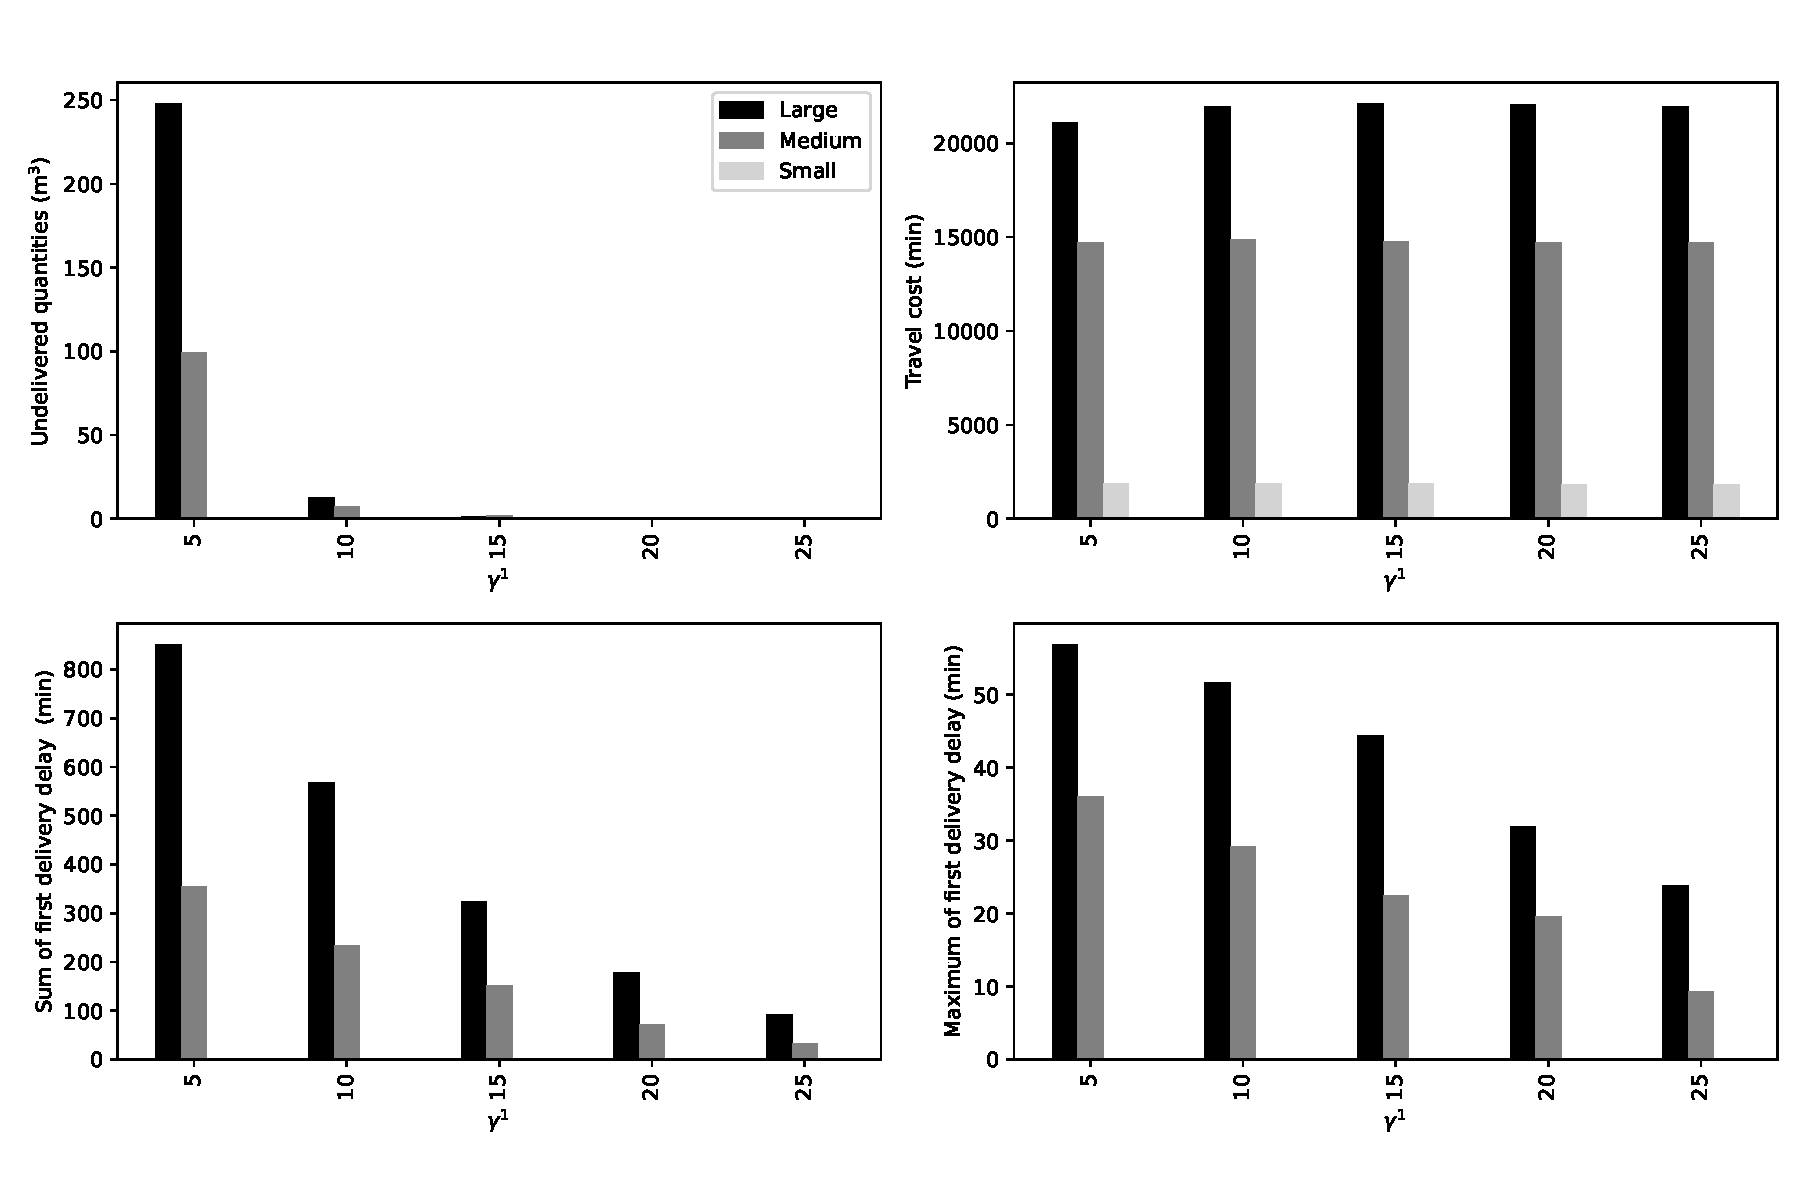
\includegraphics[width=1\textwidth]{gamma1.pdf}
    \small
    \caption{Influence of the maximum time delay ($\gamma^1$) between consecutive deliveries of the same order. }
    \label{fig:gamma1_influence}
\end{figure}

\subsubsection{Trade-off of the objective function components}

We ran five tests on our dataset and obtained two solutions per instance: one that minimizes the travel time and another that minimizes the first delivery delay. Table~\ref{tab:cdp_tradeoff} reports the trade-off between the travel time and the first delivery delay for these solutions. The difference is not noticeable for small instances. However, for medium and large instances, it is clear that as the first delivery delay decreases, the travel time increases, and conversely, when we minimize the travel time, the first delivery delay tends to be longer. This result is expected because drivers assigned to one plant often must travel to another one to ensure that the first delivery remains on schedule. This trade-off highlights the challenge decision-makers face in finding the right balance between minimizing operational costs and meeting customer satisfaction with high service levels.

\begin{table}[!ht]
    \centering
    \caption{Trade-off between travel cost and first delivery delay}
    \label{tab:cdp_tradeoff}
    \begin{adjustbox}{max width=0.8\textwidth}
    \begin{tabular}{lcccccc}
    \toprule
     & \multicolumn{3}{c}{Minimize TC} & \multicolumn{3}{c}{Minimize $FDD$} \\
     \cmidrule(l){2-4} \cmidrule(l){5-7}
     & $TC$ & $FDD$ & $mFDD$ & $TC$ & $FDD$ & $mFDD$ \\
     & (min) & (min) & (min) & (min) & (min) & (min) \\
    \midrule
    Small & 1,821.3 & 0.0 & 0.0 & 1,831.6 & 0.0 & 0.0 \\
    Medium & 14,311.5 & 89.6 & 23.0 & 14,679.3 & 46.9 & 13.4 \\
    Large & 21,403.8 & 170.5 & 31.4 & 22,194.7 & 101.7 & 29.4 \\
    \bottomrule
    \end{tabular}
\end{adjustbox}
    
\end{table}

\section{Conclusion}
\label{sec:cdp_concl}

In this paper, we investigated a variant of the concrete delivery problem, where customers can order different types of concrete from different production centers, which must be delivered during the same time window. To solve this problem, we introduced a mathematical model and a heuristic solution based on Greedy Randomized Adaptive Search. Our analysis, using a dataset derived from our partner's historical data, demonstrated the effectiveness of our algorithm in providing good solutions within a reasonable time. Furthermore, our model incorporates constraints related to working hours, making our heuristic a valuable tool for designing weekly schedules for company drivers. It can also better reassign drivers to their home plants, as these assignments affect travel costs to ensure timely deliveries. Our GRASP algorithm performed exceptionally well on the \cite{kinable2014concrete} datasets, indicating its reliability. For future work, it would be interesting to address datasets with different unloading times at construction sites or to explore different scenarios regarding the number of simultaneous deliveries and the maximum time between two consecutive orders at a construction site. One can also study the problem using a stochastic or robust methodology to account for the uncertainty of the parameters in a real-world setting. As a contribution to the literature on CDP, we provide a mathematical formulation for our variant, contribute with a dataset, and demonstrate the application of GRASP to solve both our real problem and the one studied by \cite{kinable2014concrete}.


\vspace{1.5cm} \noindent \textbf{Acknowledgments}

Financial support for this work was provided by the Canadian Natural Sciences and Engineering Research Council (NSERC) under grants 2019-00094 and 2021-04037. This support is gratefully acknowledged. We thank the Digital Research Alliance of Canada for providing high-performance computing facilities.

\bibliographystyle{plainnat}
\bibliography{references} 

\end{document}